\documentclass{beamer}
\usetheme{Madrid}
\setbeamertemplate{title page}[default][rounded=false,shadow=false]
\useoutertheme{infolines}
\usepackage[T1]{fontenc}
\usepackage{lmodern}
\usepackage{mathptmx}
\renewcommand{\rmdefault}{lmss}
\usepackage[english]{babel}
\usepackage{amsmath,amssymb,booktabs,graphicx,csquotes}
\graphicspath{{overleaf/figures/}{../figures/}}

% Preserve the existing Madrid theme and navy palette.
\definecolor{faeng_blue}{HTML}{09246F}
\definecolor{cvut_navy}{HTML}{0065BD}
\setbeamercolor*{palette primary}{bg=faeng_blue,fg=white}
\setbeamercolor*{palette secondary}{bg=faeng_blue,fg=white}
\setbeamercolor*{palette tertiary}{bg=faeng_blue,fg=white}
\setbeamercolor{titlelike}{parent=palette primary}
\setbeamercolor{frametitle}{parent=palette primary}
\setbeamercolor{itemize item}{fg=cvut_navy}
\setbeamertemplate{itemize item}[circle]
\setbeamertemplate{navigation symbols}{}
\setbeamertemplate{caption}{\raggedright\insertcaption\par}
\renewcommand{\baselinestretch}{1.15}

\title[Machine Authorship and the Review Gate]{No One to Vouch for It\\{\normalsize Machine Authorship and the Code Review Gate}}
\author[Hoang]{Minh Hoang Nguyen}
\institute[KAIST]{School of Business and Technology Management\\KAIST}
\date{Working draft: November 9, 2026}

\begin{document}
\begin{frame}[plain]
\maketitle
\end{frame}
\begin{frame}{Outline}
\tableofcontents[hideallsubsections]
\end{frame}
% =========================================================================
% part1.tex -- slide content, kept in sync with paper.tex.
% Included from slides.tex via % =========================================================================
% part1.tex -- slide content, kept in sync with paper.tex.
% Included from slides.tex via % =========================================================================
% part1.tex -- slide content, kept in sync with paper.tex.
% Included from slides.tex via \include{part1}.
%
% Active deck contains no bibliography or citation commands.
%
% New figure required:
%   figures/top1_persists_raw_event_time.png
%   (raw group means of top1_persists by event time, treated vs control)
%
% Claims deliberately removed because the data does not support them:
%   "fewer hands" / "review lands on fewer people"  -> n_reviewers is null
%   "single point of failure"                       -> top1_persists falls
% =========================================================================

\section{Motivation}

\begin{frame}{AI Changes Software Production}
\begin{itemize}
  \item RCT evidence: developers using GitHub Copilot completed a
        standardized coding task 55.8\% faster than a control group
        .
  \item Enterprise RCT: 96 Google engineers on a complex,
        enterprise-grade C++ task were about 21\% faster with AI
        assistance .
  \item Field and multi-firm evidence points the same way
        .
  \item These results motivate a production question rather than a
        universal productivity premise: what happens to code review work?
\end{itemize}
\end{frame}

\begin{frame}{The Code Review Problem}
\begin{itemize}
  \item Faster authoring means more code arriving at the review gate,
        while review itself stays human work.
  \item That code is not trustworthy by default. Across 54
        security-relevant scenarios, 44\% of the 1,084 valid programs
        Copilot produced contained a MITRE CWE
        .
  \item In a controlled user study, participants with an AI assistant
        wrote significantly less secure code than those without --- and
        were likelier to believe their code was secure
        .
  \item Bird et al.\ (GitHub / Microsoft Research) describe the same
        shift from the inside: effort moves from writing code toward
        reviewing it .
\end{itemize}
\end{frame}

\begin{frame}{Standard Pipeline}
\begin{center}
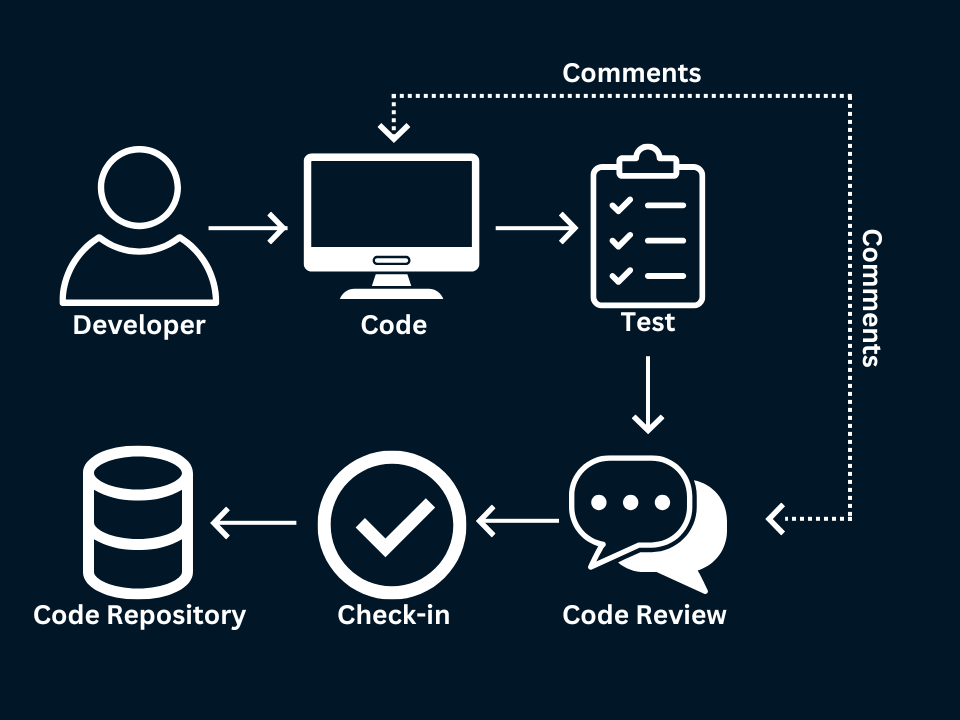
\includegraphics[width=0.6\textwidth]{code_process.png}
\end{center}
\footnotesize\centering 
Code review is where generated changes meet project knowledge,
governance, and coordination. The question is how review activity is
allocated after adoption.
\end{frame}

\section{Literature Review}

\begin{frame}{Related Work: Team-Level Effects Already Documented}
\begin{itemize}
  \item Review depth rises 5.3\% in a matched staggered-DiD study of
        11,097 repositories .
  \item Human reviewers exchange 11.8\% more rounds reviewing
        AI-generated code .
  \item An enterprise throughput mandate roughly doubles per-reviewer
        load .
\end{itemize}
\end{frame}

\begin{frame}{Related Work: Team Coordination Specifically}
\begin{itemize}
  \item AI access shifts developer time away from collaborative and
        management tasks toward solo coding, strongest for lower-skill
        developers .
  \item At Meta, lines of code per human-landed diff rose 105.9\%
        year-over-year, driven substantially by agentic AI --- review
        demand is outpacing reviewer bandwidth .
  \item Governance of AI-assisted contributions varies sharply: many
        AI-co-authored PRs merge with minimal or no human review
        .
  \item Across 1.02M pull requests, agent-involved review is faster but
        not higher-quality .
\end{itemize}
\end{frame}

\begin{frame}{Related Work: The Narrow Gap}
Closest comparator: Copilot adoption raises project-level contributions
5.9\% and coordination time 8\%; core-developer reviews, reviews per
core developer, and distinct core reviewers all rise
.
\vspace{0.3em}
\textbf{The remaining question here:}
\begin{itemize}
  \item Project-level averages and counts do not reveal the distribution
        of review activity across people.
  \item Monthly concentration and fixed reviewer identity are distinct:
        the busiest people can change while concentration stays constant.
  \item We study review-share concentration jointly with continuity of
        the people occupying leading review positions.
\end{itemize}
\end{frame}

\section{Theory}

% \begin{frame}{Review as a Transactive Memory System}
% A transactive memory system (TMS) is a group's shared directory of
% \emph{who knows what} -- members specialize, and the group knows whom
% to route a problem to .
% \begin{itemize}
%   \item In software, that directory is built from accumulated codebase
%         memory: why a decision was made, what broke before.
%   \item Review is where it's exercised -- who reviews what determines
%         what gets caught.
%   \item Open-source review makes it \textbf{observable}: assignment is
%         recorded behaviour, not survey data.
% \end{itemize}
% \vspace{0.3em}
% TMS separates two things the throughput literature conflates: how
% \emph{specialized} code review is, and \emph{whom} it's specialized
% onto.
% \end{frame}



% \begin{frame}{The Review Process, Before AI}
% \begin{center}
% 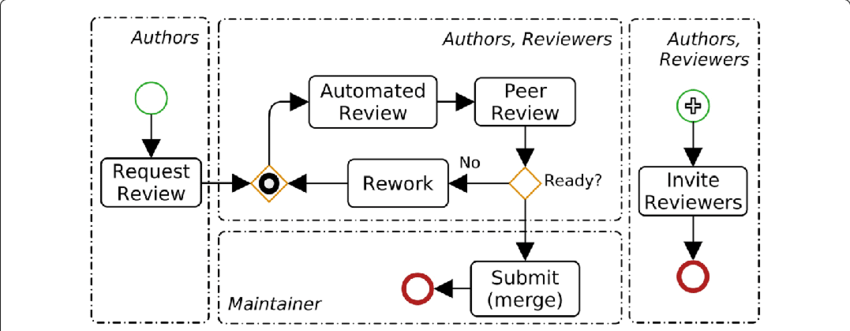
\includegraphics[width=0.78\textwidth]{review_process.png}
% \end{center}
% \footnotesize\centering Inside ``Code Review''
% \\
% \vspace{0.5em}
% \end{frame}

\begin{frame}{Research Questions}
\textbf{Question:} when a repository first exhibits an AI-adoption
signal, how does its review work reorganize?
\begin{enumerate}
  \item[RQ1] Does the distribution of monthly review activity change?
  \item[RQ2] Does the pre-adoption leading reviewer remain in the leading
        position, and what happens to successor stability?
  \item[RQ3] What process outcomes accompany these allocation patterns?
\end{enumerate}
\end{frame}

\section{Research Design and Data}

\begin{frame}{Research Design}
\begin{itemize}
  \item Treatment: a repository's own AI-tool adoption, $t_0$ =
        earliest detected signal.
  \item Staggered-adoption DiD on covariate-matched treated/control
        repositories.
  \item Imputation estimator of  ---
        avoids the ``forbidden comparisons'' bias of naive two-way
        fixed effects under staggered timing
        .
  \item 1,771 matched pairs, 20,188 repository-month observations.
\end{itemize}
\end{frame}

\begin{frame}{Data Construction}
\begin{itemize}
  \item 8,972 candidate repositories, stratified across 6 languages
        $\times$ 4 creation-year cohorts, quality-filtered ($\geq$10
        stars, not a fork, minimum contributor count, recent activity
        ).
  \item AI-adoption signal (OR-combined): autonomous agent PR
        authorship, commit co-authorship trailers, configuration-file
        presence. $t_0$ = first detected signal of any kind.
  \item[] 8,972 candidates $\rightarrow$ 2,320 matched pairs (caliper
        0.25 SD) $\rightarrow$ 1,771 pairs with complete panel data.
\end{itemize}
\end{frame}

\begin{frame}{Outcome Variables}
Each measured per repository-month; construction detail in backup.
\begin{itemize}
  \item \textbf{Specialization:} top1\_share/top2\_share -- the busiest
        one/two reviewers' share of a repo-month's total human review
        activity; tail\_share is the complement held by everyone else.
  \item \textbf{Directory assignment:} top1\_persists: is this month's
        busiest reviewer the same person as the repository's fixed
        pre-period top-1? Same for the top-2 pair.
\end{itemize}
\end{frame}

\begin{frame}{Outcome Variables}
Gini coefficient over a repo-month's full reviews-per-reviewer
distribution: 
\[
G_{it}=\frac{\displaystyle\sum_{r=1}^{n}\sum_{q=1}^{n}
\left|x_{rit}-x_{qit}\right|}
{\displaystyle 2n\sum_{r=1}^{n}x_{rit}}
\]
\begin{itemize}
  \item $x_i$ = number of reviews reviewer $i$ submitted that
        repo-month; $n$ = number of distinct human reviewers that
        repo-month.
  \item G = 0 mean every reviewer handled an equal share.
  \item G = 1 mean one reviewer handled all of it.
\end{itemize}
\end{frame}

\section{Empirical Strategy}

\begin{frame}{Introducing BJS: Why We Need It}
\begin{itemize}
  \item Repos adopt AI at different times --- naive two-way fixed
        effects implicitly compares late adopters against
        already-treated early adopters, not just never-treated
        controls.
  \item These ``forbidden comparisons'' bias the estimate whenever the
        treatment effect changes over time
         --- exactly our case, since our
        effects grow across the post-period.
  \item We use the imputation estimator of
         (``BJS''): it builds each treated
        repo's counterfactual only from never-yet-treated data, so an
        already-treated repo can never contaminate another's
        comparison.
\end{itemize}
\end{frame}

\begin{frame}{Estimator}
Two-step imputation :
\begin{enumerate}
  \item Fit $y_{it}=\alpha_i+\beta_t+\varepsilon_{it}$ on $\Omega_0$
        (controls' full history + treated repos' pre-$t_0$
        observations only).
  \item Predict $\hat y_{it}(0)=\hat\alpha_i+\hat\beta_t$ for treated
        post-$t_0$ observations; $\text{ATT}_h$ = mean residual at
        event-time horizon $h$.
\end{enumerate}
\vspace{0.5em}
Event time: pre-leads $h=-6,\dots,-2$ (no-anticipation: $h=-1$
excluded), post-period $h=0,\dots,11$.
\vspace{0.5em}
Post-adoption data = a treated repo's own observations after its $t_0$.
Step 1 never uses it.
\end{frame}

\begin{frame}{BJS in Practice: Observed vs.\ Counterfactual}
\begin{center}
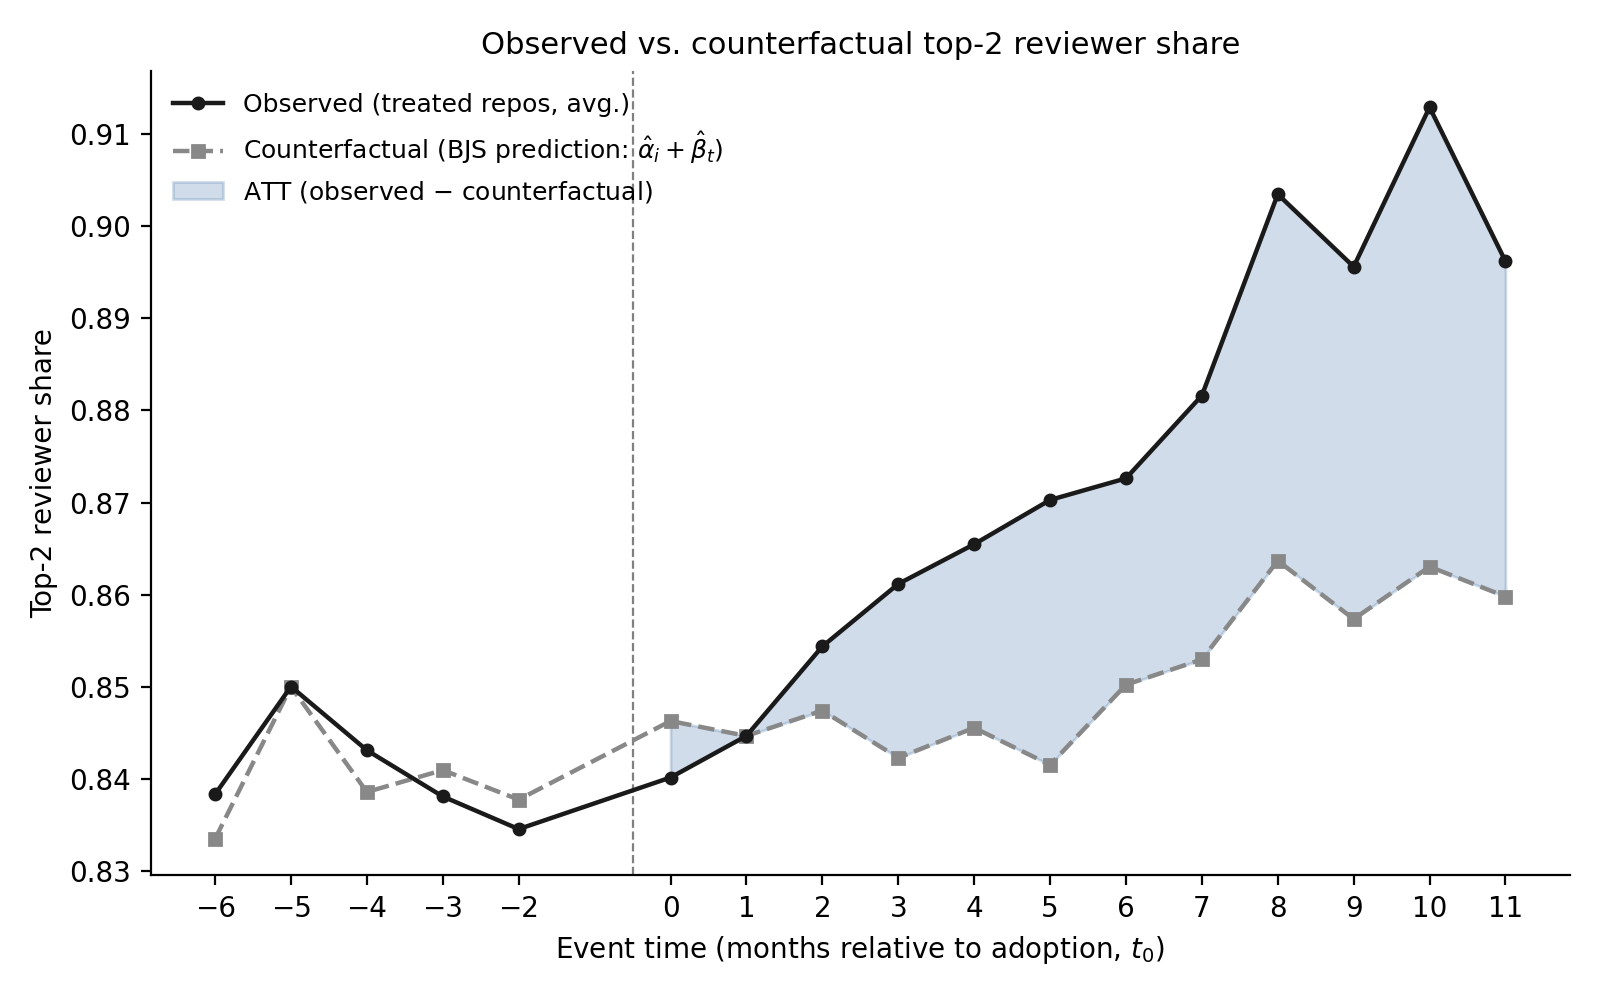
\includegraphics[width=0.85\textwidth]{bjs_illustration_top2_share.png}
\end{center}
\end{frame}

\section{Results}

\begin{frame}{RQ1 --- Monthly Review Activity Becomes More Concentrated}
\begin{table}
\centering
\small
\begin{tabular}{lrr}
\toprule
Outcome & ATT & $p$ \\
\midrule
Top-1 review share & $+0.017$ \ (0.0089) & 0.052 \\
Top-2 review share & $+0.015^{**}$ \ (0.0050) & 0.003 \\
Tail share (outside the top two) & $-0.015^{***}$ & $<0.001$ \\
Reviewer Gini coefficient & $+0.030^{***}$ & $<0.001$ \\
\addlinespace
\multicolumn{3}{l}{\textit{Repos with 3+ reviewers monthly}} \\
Top-1 review share & $+0.041^{***}$ \ (0.0072) & $<0.001$ \\
Top-2 review share & $+0.036^{***}$ \ (0.0052) & $<0.001$ \\
\addlinespace
Repo FE & Yes & \\
Time FE & Yes & \\
\bottomrule
\end{tabular}
\end{table}
\end{frame}

\begin{frame}{RQ1 --- What the Numbers Show}
\begin{itemize}
  \item \textbf{Headcount:} team size is unchanged in this outcome -- the
        observed distribution changes within the measured reviewer set.
  \item \textbf{Concentration:} top-2 share rises while tail share falls
        by almost the same amount, and the Gini rises across the whole
        distribution.
  \item Many repo-months start pinned near 100\% (only 1--2 reviewers),
        diluting the pooled estimate; restricting to 3+ reviewers
        roughly doubles it.
\end{itemize}
\vspace{0.3em}
\end{frame}

\begin{frame}{RQ1 --- Concentration Depends on Whether Leadership Was Already Settled}
Split treated repos by whether one person already held the top spot for
the entire 5-month pre-period (``settled'') or not (``unsettled''):
\begin{table}
\centering
\small
\begin{tabular}{lrr}
\toprule
Outcome & Unsettled leader ($n{=}191$) & Settled leader ($n{=}105$) \\
\midrule
Top-1 review share & $+0.047$ (4.62) & $-0.022$ ($-1.84$) \\
Top-2 review share & $+0.036$ (4.40) & $+0.001$ (0.14) \\
\bottomrule
\end{tabular}
\end{table}
\begin{itemize}
  \item Both strata pass pre-trend cleanly; the difference between them
        is strongly significant (top-1: $p<0.0001$, top-2: $p=0.003$).
  \item \textbf{Scope:} this subsample (complete 5-month pre-period
        coverage) also skews busier than average ($\sim$2$\times$ the
        pre-period PR volume)
\end{itemize}
\end{frame}

\begin{frame}{RQ2 --- Incumbent Persistence Falls}
\begin{table}
\centering
\small
\begin{tabular}{lrr}
\toprule
Outcome & ATT & $p$ \\
\midrule
Monthly leader is the pre-adoption top-1 & $-0.077^{***}$ \ (0.0151) & $<0.001$ \\
Monthly top-2 overlaps the pre-adoption top-2 & $-0.045^{***}$ \ (0.0101) & $<0.001$ \\
Month-to-month leader change & $-0.058^{**}$ \ (0.0197) & 0.004 \\
\addlinespace
Repo FE & Yes & \\
Time FE & Yes & \\
\bottomrule
\end{tabular}
\end{table}
\begin{itemize}
  \item The pre-adoption lead is less likely to remain the monthly leader
        after adoption.
\end{itemize}
\end{frame}

\begin{frame}{RQ2 --- Is the Persistence Result a Construction Artifact?}
The fixed identity is chosen by taking the maximum over
$h=-6,\dots,-2$, and those same months form the estimation baseline ---
which inflates pre-period persistence by construction.
\begin{center}
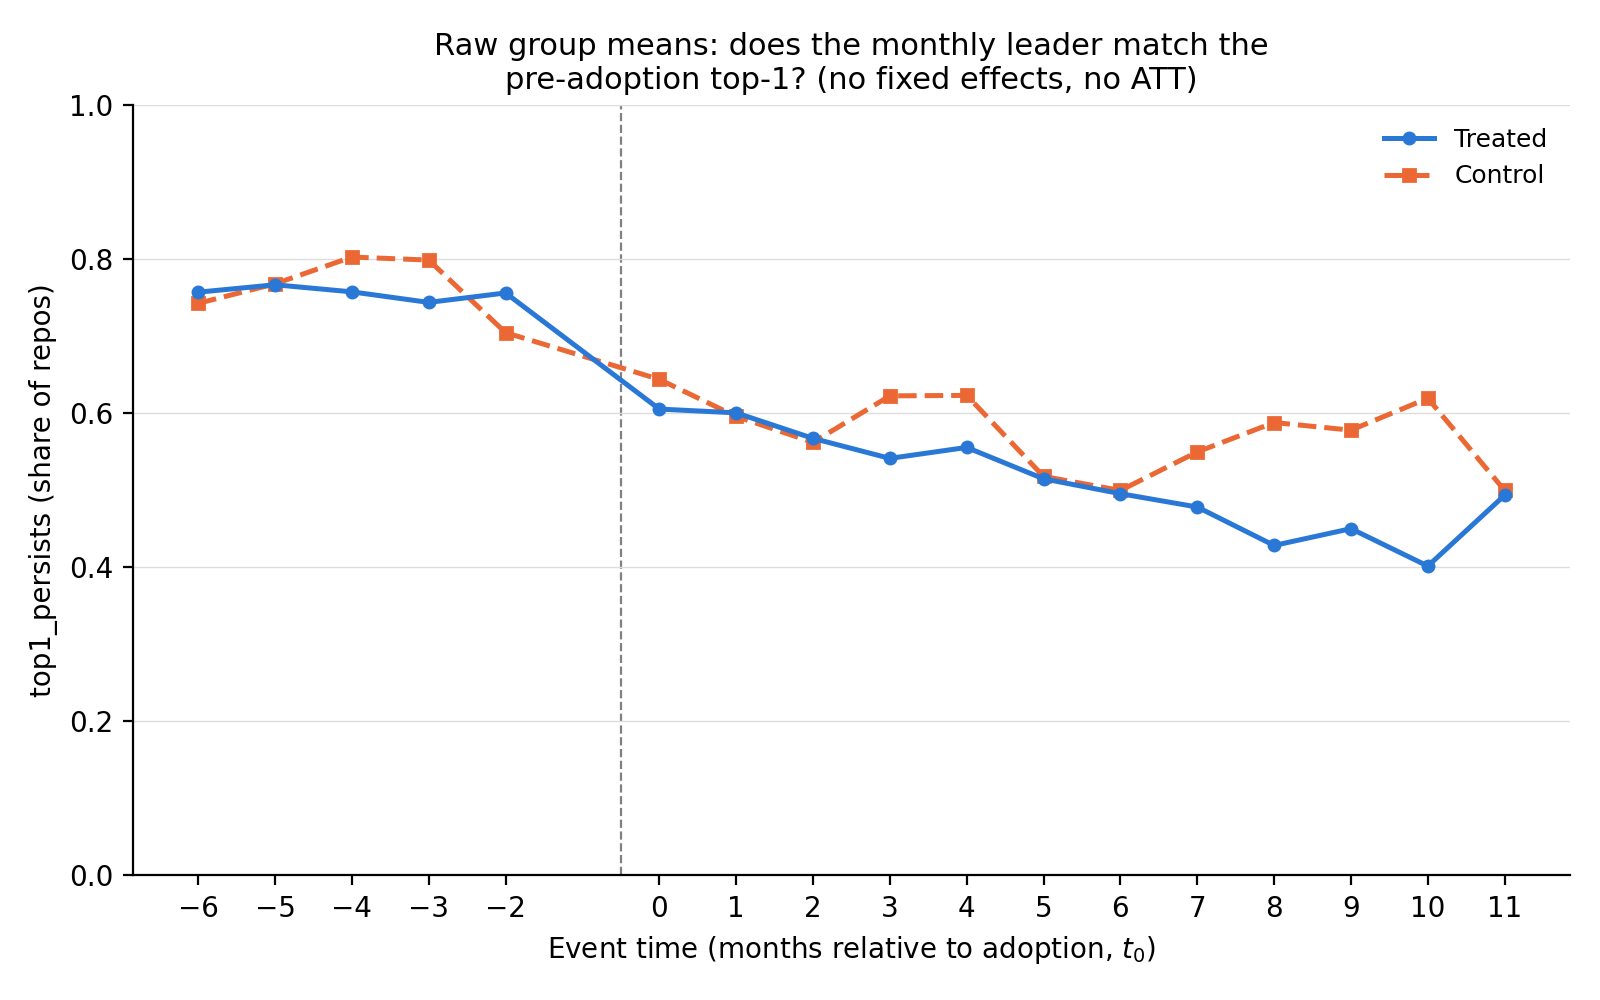
\includegraphics[width=0.62\textwidth]{top1_persists_raw_event_time.png}
\end{center}
\vspace{-0.3em}
\footnotesize Both groups drop from $\sim$0.75 to $\sim$0.60 at
$h\!=\!0$. Because the drop is common to treated and control, the
difference-in-differences nets it out; the series separate only later.
\end{frame}

\begin{frame}{RQ3 --- Process Outcomes}
\begin{table}
\centering
\small
\begin{tabular}{lrr}
\toprule
Outcome & ATT & $p$ \\
\midrule
Time to first review (h) & $-65.0^{*}$ \ (28.91) & 0.025 \\
Time to merge (h)        & $-62.8^{*}$ \ (27.10) & 0.021 \\
Review rounds/PR         & $+0.180^{*}$ \ (0.082) & 0.027 \\
\addlinespace
Repo FE & Yes & \\
Time FE & Yes & \\
\bottomrule
\end{tabular}
\end{table}
\begin{itemize}
  \item PRs reach a first recorded review and merge sooner, while review
        submissions per PR increase.
\end{itemize}
\end{frame}

\begin{frame}{H3 --- Do Pull Requests Just Get Smaller?}
\begin{table}
\centering
\small
\begin{tabular}{lrr}
\toprule
Spec & ATT (hours) & $t$ \\
\midrule
Unrestricted (uncapped PR-level data) & $-34.2$ & $-1.74$ \\
Residualized on PR size & $-35.8$ & $-1.82$ \\
Restricted to similarly-sized PRs (25th--75th pct.) & $-61.8$ & $-2.62$ \\
\bottomrule
\end{tabular}
\end{table}
\begin{itemize}
  \item With PR size held fixed, latency still falls --- merges get
        faster, not merely smaller.
\end{itemize}
\end{frame}

\begin{frame}{H3 --- Reverses in Busy Repos}
On the busier-than-average subsample ($\sim$2$\times$ pre-period PR
volume, $n{=}296$):
\begin{table}
\centering
\small
\begin{tabular}{lrr}
\toprule
Outcome & Full sample & Busy subsample \\
\midrule
Time to merge (h) & $-62.8$ (2.60) & $+40.7$ (2.83) \\
Review rounds/PR & $+0.180$ (4.04) & $-0.146$ (2.04) \\
\bottomrule
\end{tabular}
\end{table}
\begin{itemize}
  \item Both directions pass pre-trends in both samples; the full
        sample's own $\text{ATT}_h$ never flips sign across horizons.
  \item In high-volume repos, merging gets \textbf{slower} and needs
        \textbf{fewer} rounds after adoption, the opposite pattern from
        the general sample.
\end{itemize}
\end{frame}

\section{Discussion}
\begin{frame}{Discussion}
Our results suggest a reallocation of review authority, with important
limits on what the data can identify.
\begin{itemize}
  \item The pre-adoption leader is less likely to remain first after
        adoption, while monthly concentration can rise.
  \item Reassignment is stronger where leadership was not already
        settled, but that pattern is confounded with baseline activity.
  \item The data do not show whether successors have less context or
        whether incumbents face more absolute work.
\end{itemize}
\vspace{0.3em}
The supported claim is a change in observed allocation and continuity,
not a proven loss of expertise or durable authority.
\end{frame}

\begin{frame}{Reconstructing the Process}
The standard pipeline (earlier slide) treats code review as a
discrete gate at the end: write, then check. That shape assumes
writing is the slow, scarce step.
\begin{itemize}
  \item AI-assisted production changes the volume and composition of work
        reaching review, while the organizational response remains an
        empirical question.
  \item The observed evidence points to a change in review allocation and
        incumbent continuity, with substantial sample and measurement
        sensitivity.
  \item The data do not identify whether successors have less context,
        whether incumbents face more absolute work, or whether quality
        improves or declines.
\end{itemize}
\vspace{0.3em}
The supported contribution is a measurement framework for studying
allocation, continuity, and process timing together.
\end{frame}

\begin{frame}{Are Our Controls Actually Independent?}
\textbf{Problem:} 37.7\% of repos share a human reviewer with some
treated repo elsewhere in the sample -- that reviewer can carry
AI-adoption habits into a repo we're counting as an untreated
``control,'' violating the no-interference assumption the design needs.
\vspace{0.3em}

\textbf{What we did:} identified 176 pairs without observed reviewer
overlap and examined the headline outcomes in that restricted sample.
\vspace{0.3em}

\textbf{Result if contamination is removed:}
\begin{itemize}
  \item Top-2 share and incumbent persistence retain their direction;
        the persistence estimate is larger in the restricted sample.
  \item Other outcomes weaken or become imprecise, as expected after the
        population is reduced to 176 pairs.
  \item Month-to-month leader-change rate collapses to $t{\approx}0$ and
        is dropped as a robust claim.
\end{itemize}
\end{frame}

\begin{frame}{Is the Reported Inference Trustworthy?}
Analytic cluster-robust SE vs.\ a 300-replicate repo-pair bootstrap:
\begin{table}
\centering
\scriptsize
\begin{tabular}{lrrrr}
\toprule
Outcome & Analytic SE & Bootstrap SE & Ratio & Corrected $p$ \\
\midrule
Top-1 review share     & 0.0064 & 0.0089 & 1.39$\times$ & 0.052 \\
Top-2 review share     & 0.0034 & 0.0050 & 1.45$\times$ & 0.003 \\
Time to first review   & 21.40  & 28.91  & 1.35$\times$ & 0.025 \\
Time to merge          & 24.18  & 27.10  & 1.12$\times$ & 0.021 \\
Review rounds          & 0.045  & 0.082  & 1.83$\times$ & 0.027 \\
\bottomrule
\end{tabular}
\end{table}
The analytic SE understates true uncertainty by 12--83\%. Top-1 share
drops to borderline ($p=0.052$); everything else survives. All tables
in this deck use the corrected $p$.
\end{frame}

\begin{frame}{The Parallel-Trends Assumption for BJS}
\begin{itemize}
  \item BJS builds each treated repo's counterfactual,
        $\hat\alpha_i+\hat\beta_t$, from a model fit only on
        pre-adoption and control data. That counterfactual is valid
        only if, absent treatment, the repo would have kept following
        that same repo-baseline-plus-calendar-trend path.
  \item Primary check (go/no-go): joint Wald test on the five
        pre-period lead coefficients ($h=-6,\dots,-2$), $\chi^2_5$.
  \item Secondary check (margin of safety): how large an undetected
        pre-trend would need to be, extrapolated forward, to explain
        away the post-period effect --- in units of the estimated
        pre-trend's own SE.
\end{itemize}
\begin{table}
\centering
\tiny
\begin{tabular}{lr}
\toprule
Outcome & Breakdown slope, in SE units \\
\midrule
Top-1 review share     & 2.6$\times$ (wrong-signed pre-trend --- helps us) \\
Top-2 review share     & 3.4$\times$ (wrong-signed pre-trend --- helps us) \\
Time to first review   & 3.7$\times$ (same-signed --- erodes $\sim$36\% of ATT) \\
Time to merge          & 3.8$\times$ \\
Review rounds          & 3.0$\times$ (same-signed --- erodes $\sim$55\% of ATT) \\
\bottomrule
\end{tabular}
\end{table}
\end{frame}

\begin{frame}{Does the Effect Differ by Adoption Era?}
Repos adopted 2025-05 to 2025-11 (``Era 2'', $n{=}413$) vs.\
2025-11 to 2026-05 (``Era 3'', $n{=}666$) -- the two best-powered
calendar-time cohorts, roughly bracketing successive generations of
agentic coding tools:
\begin{table}
\centering
\small
\begin{tabular}{lrrl}
\toprule
Outcome & Era 2 ATT & Era 3 ATT & Diff.\ test \\
\midrule
Top-1 review share & $+0.028$ & $+0.020$ & $p=0.60$ \\
Top-2 review share & $+0.021$ & $+0.014$ & $p=0.42$ \\
\bottomrule
\end{tabular}
\end{table}
\begin{itemize}
  \item No test in a full battery -- caliper sensitivity, bootstrap
        SE, clean-sample restriction -- ever produces a significant
        Era-2-vs-Era-3 difference on this comparison.
  \item \textbf{The effect is not detectably different across adoption
        eras.} Not driven by a specific generation of AI coding tools.
\end{itemize}
\end{frame}

\begin{frame}{Does the Effect Differ by Specific Tool?}
Beyond agent-vs-assisted MODE (earlier slide): does it matter whether a
repo adopted Codex, Copilot, Claude, or Cursor specifically? Buckets are
non-exclusive (a repo can carry signals for more than one tool).
\begin{table}
\centering
\small
\begin{tabular}{lrrr}
\toprule
Tool ($n$) & Top-2 share $t$ & Time-to-merge $t$ \\
\midrule
Codex (961)    & $+1.57$ & $-2.97$ \\
Copilot (800)  & $+3.18$ & $-2.60$ \\
Claude (478)   & $+2.55$ & $-1.26$ \\
Cursor (151)   & $+0.66$ & $+1.10$ \\
\bottomrule
\end{tabular}
\end{table}
\vspace{0.2em}
\textbf{Conclusion:} the concentration result is not detectably different
across adoption eras or specific AI tools; Codex's latency estimate is
individually robust but not larger than the alternatives.
\end{frame}

% \begin{frame}{Robustness: Extraction Cap and Common Horizon}
% \begin{table}
% \centering\small
% \begin{tabular}{lrr}
% \toprule
% Top-two share specification & ATT & Notes \\
% \midrule
% Original capped extraction & $+0.0153$ & full eligible sample \\
% Uncapped extraction & $+0.0082$ & same 802-repository subsample \\
% Full event window & $+0.0151$ & pooled sample \\
% Common horizon $h=0,\ldots,5$ & $+0.0081$ & fixed early window \\
% \bottomrule
% \end{tabular}
% \end{table}
% \begin{itemize}
%   \item Direction is stable, but magnitude depends on the extraction cap
%         and the changing cohort composition at longer horizons.
%   \item The cap and common-horizon checks limit a strong claim about the
%         size of the concentration effect.
% \end{itemize}
% \end{frame}

\begin{frame}{Robustness: No Observed Reviewer Overlap}
\begin{table}
\centering\scriptsize
\begin{tabular}{lrr}
\toprule
Outcome, 176 pairs & ATT & Analytic $t$ \\
\midrule
Top-one share & $+0.0118$ & 0.86 \\
Top-two share & $+0.0208$ & 2.79 \\
Incumbent persistence & $-0.1106$ & $-3.70$ \\
Pre-adoption top-two overlap & $+0.0095$ & 0.45 \\
Monthly leader changes & $-0.0006$ & $-0.02$ \\
First recorded review (h) & $-89.77$ & $-2.92$ \\
Merge time (h) & $-56.15$ & $-1.88$ \\
Review submissions/PR & $+0.1756$ & 1.82 \\
\bottomrule
\end{tabular}
\end{table}
\footnotesize This restriction changes the population and uses analytic
inference, not the pooled table's bootstrap. It removes observed overlap,
not every possible spillover.
\end{frame}


\begin{frame}[plain]
\begin{center}
\Large Thank you
\vspace{1em}

\normalsize Questions?
\end{center}
\end{frame}
.
%
% Active deck contains no bibliography or citation commands.
%
% New figure required:
%   figures/top1_persists_raw_event_time.png
%   (raw group means of top1_persists by event time, treated vs control)
%
% Claims deliberately removed because the data does not support them:
%   "fewer hands" / "review lands on fewer people"  -> n_reviewers is null
%   "single point of failure"                       -> top1_persists falls
% =========================================================================

\section{Motivation}

\begin{frame}{AI Changes Software Production}
\begin{itemize}
  \item RCT evidence: developers using GitHub Copilot completed a
        standardized coding task 55.8\% faster than a control group
        .
  \item Enterprise RCT: 96 Google engineers on a complex,
        enterprise-grade C++ task were about 21\% faster with AI
        assistance .
  \item Field and multi-firm evidence points the same way
        .
  \item These results motivate a production question rather than a
        universal productivity premise: what happens to code review work?
\end{itemize}
\end{frame}

\begin{frame}{The Code Review Problem}
\begin{itemize}
  \item Faster authoring means more code arriving at the review gate,
        while review itself stays human work.
  \item That code is not trustworthy by default. Across 54
        security-relevant scenarios, 44\% of the 1,084 valid programs
        Copilot produced contained a MITRE CWE
        .
  \item In a controlled user study, participants with an AI assistant
        wrote significantly less secure code than those without --- and
        were likelier to believe their code was secure
        .
  \item Bird et al.\ (GitHub / Microsoft Research) describe the same
        shift from the inside: effort moves from writing code toward
        reviewing it .
\end{itemize}
\end{frame}

\begin{frame}{Standard Pipeline}
\begin{center}
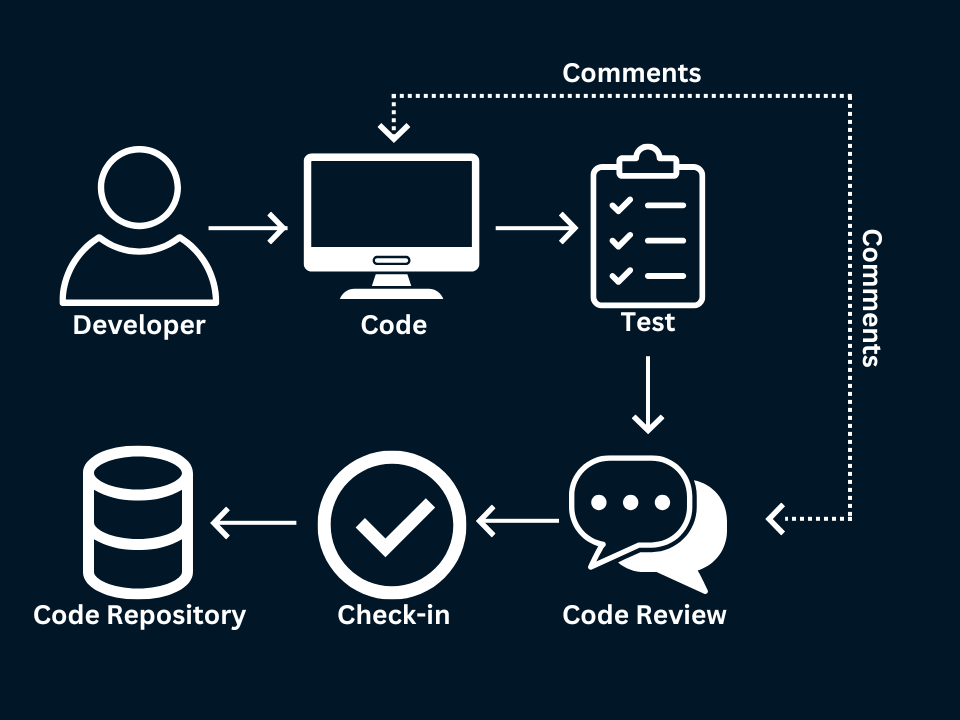
\includegraphics[width=0.6\textwidth]{code_process.png}
\end{center}
\footnotesize\centering 
Code review is where generated changes meet project knowledge,
governance, and coordination. The question is how review activity is
allocated after adoption.
\end{frame}

\section{Literature Review}

\begin{frame}{Related Work: Team-Level Effects Already Documented}
\begin{itemize}
  \item Review depth rises 5.3\% in a matched staggered-DiD study of
        11,097 repositories .
  \item Human reviewers exchange 11.8\% more rounds reviewing
        AI-generated code .
  \item An enterprise throughput mandate roughly doubles per-reviewer
        load .
\end{itemize}
\end{frame}

\begin{frame}{Related Work: Team Coordination Specifically}
\begin{itemize}
  \item AI access shifts developer time away from collaborative and
        management tasks toward solo coding, strongest for lower-skill
        developers .
  \item At Meta, lines of code per human-landed diff rose 105.9\%
        year-over-year, driven substantially by agentic AI --- review
        demand is outpacing reviewer bandwidth .
  \item Governance of AI-assisted contributions varies sharply: many
        AI-co-authored PRs merge with minimal or no human review
        .
  \item Across 1.02M pull requests, agent-involved review is faster but
        not higher-quality .
\end{itemize}
\end{frame}

\begin{frame}{Related Work: The Narrow Gap}
Closest comparator: Copilot adoption raises project-level contributions
5.9\% and coordination time 8\%; core-developer reviews, reviews per
core developer, and distinct core reviewers all rise
.
\vspace{0.3em}
\textbf{The remaining question here:}
\begin{itemize}
  \item Project-level averages and counts do not reveal the distribution
        of review activity across people.
  \item Monthly concentration and fixed reviewer identity are distinct:
        the busiest people can change while concentration stays constant.
  \item We study review-share concentration jointly with continuity of
        the people occupying leading review positions.
\end{itemize}
\end{frame}

\section{Theory}

% \begin{frame}{Review as a Transactive Memory System}
% A transactive memory system (TMS) is a group's shared directory of
% \emph{who knows what} -- members specialize, and the group knows whom
% to route a problem to .
% \begin{itemize}
%   \item In software, that directory is built from accumulated codebase
%         memory: why a decision was made, what broke before.
%   \item Review is where it's exercised -- who reviews what determines
%         what gets caught.
%   \item Open-source review makes it \textbf{observable}: assignment is
%         recorded behaviour, not survey data.
% \end{itemize}
% \vspace{0.3em}
% TMS separates two things the throughput literature conflates: how
% \emph{specialized} code review is, and \emph{whom} it's specialized
% onto.
% \end{frame}



% \begin{frame}{The Review Process, Before AI}
% \begin{center}
% 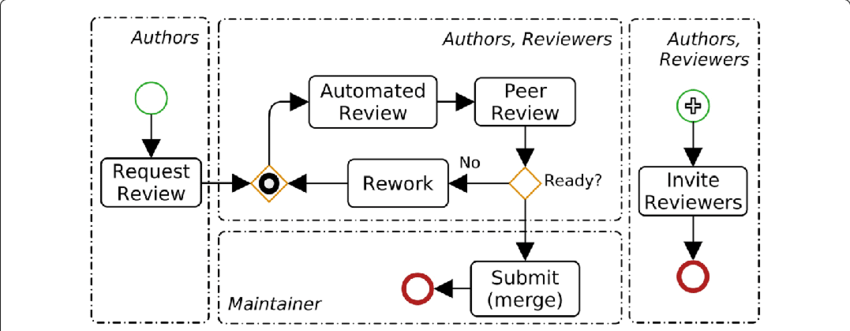
\includegraphics[width=0.78\textwidth]{review_process.png}
% \end{center}
% \footnotesize\centering Inside ``Code Review''
% \\
% \vspace{0.5em}
% \end{frame}

\begin{frame}{Research Questions}
\textbf{Question:} when a repository first exhibits an AI-adoption
signal, how does its review work reorganize?
\begin{enumerate}
  \item[RQ1] Does the distribution of monthly review activity change?
  \item[RQ2] Does the pre-adoption leading reviewer remain in the leading
        position, and what happens to successor stability?
  \item[RQ3] What process outcomes accompany these allocation patterns?
\end{enumerate}
\end{frame}

\section{Research Design and Data}

\begin{frame}{Research Design}
\begin{itemize}
  \item Treatment: a repository's own AI-tool adoption, $t_0$ =
        earliest detected signal.
  \item Staggered-adoption DiD on covariate-matched treated/control
        repositories.
  \item Imputation estimator of  ---
        avoids the ``forbidden comparisons'' bias of naive two-way
        fixed effects under staggered timing
        .
  \item 1,771 matched pairs, 20,188 repository-month observations.
\end{itemize}
\end{frame}

\begin{frame}{Data Construction}
\begin{itemize}
  \item 8,972 candidate repositories, stratified across 6 languages
        $\times$ 4 creation-year cohorts, quality-filtered ($\geq$10
        stars, not a fork, minimum contributor count, recent activity
        ).
  \item AI-adoption signal (OR-combined): autonomous agent PR
        authorship, commit co-authorship trailers, configuration-file
        presence. $t_0$ = first detected signal of any kind.
  \item[] 8,972 candidates $\rightarrow$ 2,320 matched pairs (caliper
        0.25 SD) $\rightarrow$ 1,771 pairs with complete panel data.
\end{itemize}
\end{frame}

\begin{frame}{Outcome Variables}
Each measured per repository-month; construction detail in backup.
\begin{itemize}
  \item \textbf{Specialization:} top1\_share/top2\_share -- the busiest
        one/two reviewers' share of a repo-month's total human review
        activity; tail\_share is the complement held by everyone else.
  \item \textbf{Directory assignment:} top1\_persists: is this month's
        busiest reviewer the same person as the repository's fixed
        pre-period top-1? Same for the top-2 pair.
\end{itemize}
\end{frame}

\begin{frame}{Outcome Variables}
Gini coefficient over a repo-month's full reviews-per-reviewer
distribution: 
\[
G_{it}=\frac{\displaystyle\sum_{r=1}^{n}\sum_{q=1}^{n}
\left|x_{rit}-x_{qit}\right|}
{\displaystyle 2n\sum_{r=1}^{n}x_{rit}}
\]
\begin{itemize}
  \item $x_i$ = number of reviews reviewer $i$ submitted that
        repo-month; $n$ = number of distinct human reviewers that
        repo-month.
  \item G = 0 mean every reviewer handled an equal share.
  \item G = 1 mean one reviewer handled all of it.
\end{itemize}
\end{frame}

\section{Empirical Strategy}

\begin{frame}{Introducing BJS: Why We Need It}
\begin{itemize}
  \item Repos adopt AI at different times --- naive two-way fixed
        effects implicitly compares late adopters against
        already-treated early adopters, not just never-treated
        controls.
  \item These ``forbidden comparisons'' bias the estimate whenever the
        treatment effect changes over time
         --- exactly our case, since our
        effects grow across the post-period.
  \item We use the imputation estimator of
         (``BJS''): it builds each treated
        repo's counterfactual only from never-yet-treated data, so an
        already-treated repo can never contaminate another's
        comparison.
\end{itemize}
\end{frame}

\begin{frame}{Estimator}
Two-step imputation :
\begin{enumerate}
  \item Fit $y_{it}=\alpha_i+\beta_t+\varepsilon_{it}$ on $\Omega_0$
        (controls' full history + treated repos' pre-$t_0$
        observations only).
  \item Predict $\hat y_{it}(0)=\hat\alpha_i+\hat\beta_t$ for treated
        post-$t_0$ observations; $\text{ATT}_h$ = mean residual at
        event-time horizon $h$.
\end{enumerate}
\vspace{0.5em}
Event time: pre-leads $h=-6,\dots,-2$ (no-anticipation: $h=-1$
excluded), post-period $h=0,\dots,11$.
\vspace{0.5em}
Post-adoption data = a treated repo's own observations after its $t_0$.
Step 1 never uses it.
\end{frame}

\begin{frame}{BJS in Practice: Observed vs.\ Counterfactual}
\begin{center}
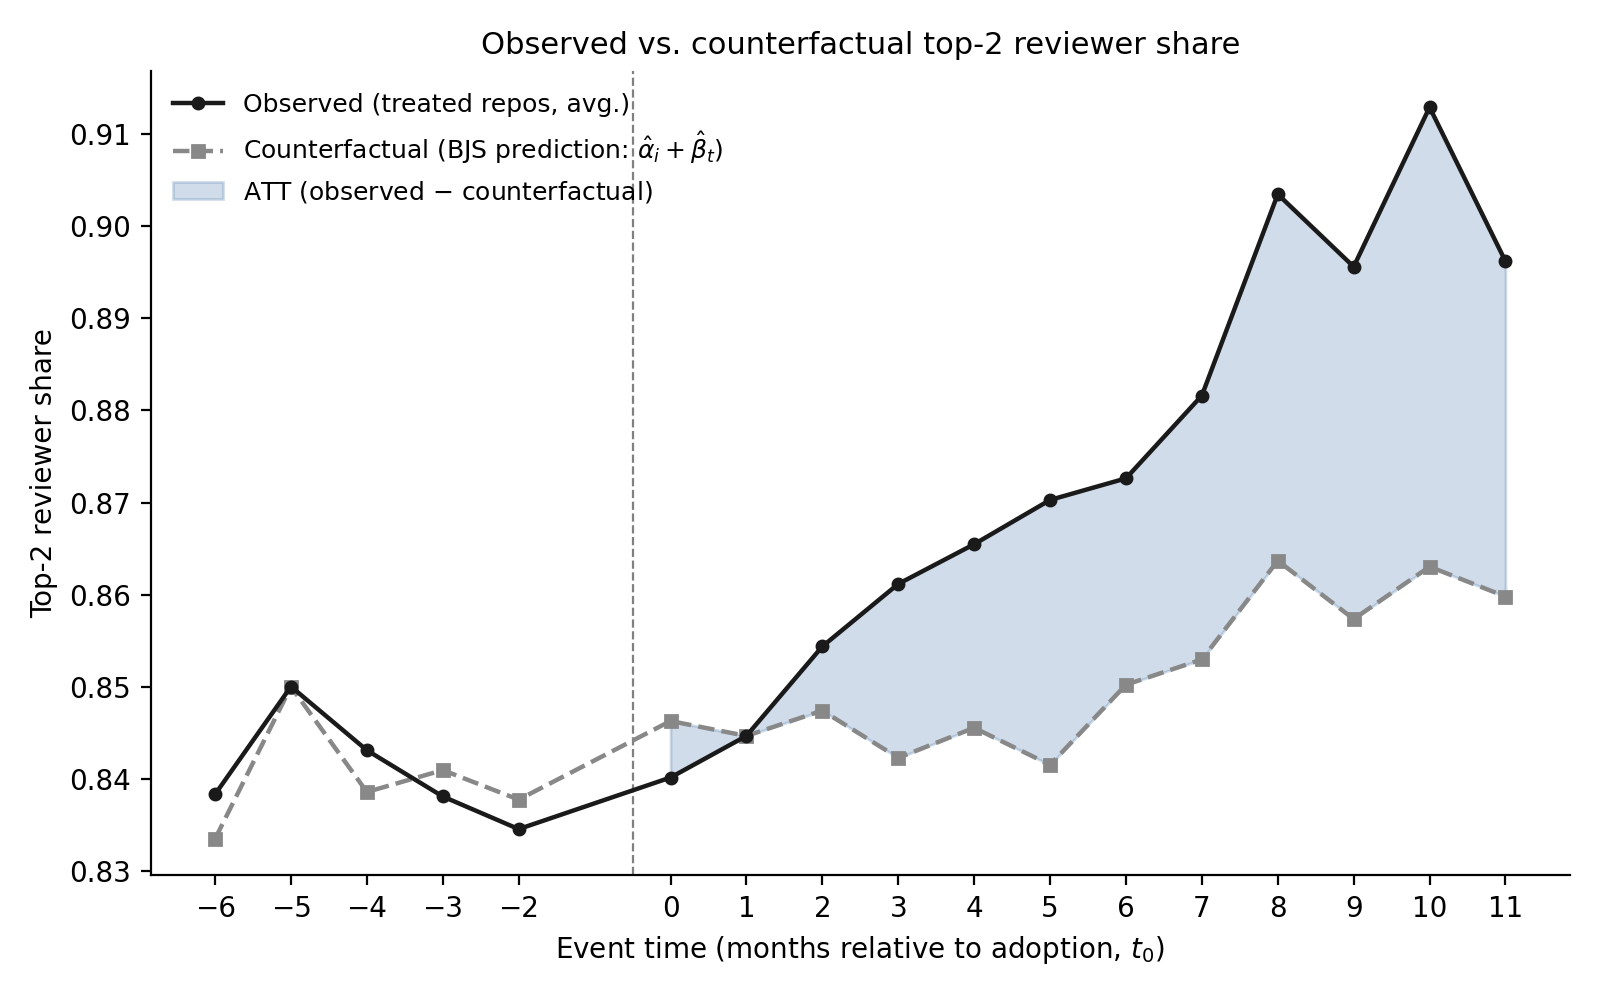
\includegraphics[width=0.85\textwidth]{bjs_illustration_top2_share.png}
\end{center}
\end{frame}

\section{Results}

\begin{frame}{RQ1 --- Monthly Review Activity Becomes More Concentrated}
\begin{table}
\centering
\small
\begin{tabular}{lrr}
\toprule
Outcome & ATT & $p$ \\
\midrule
Top-1 review share & $+0.017$ \ (0.0089) & 0.052 \\
Top-2 review share & $+0.015^{**}$ \ (0.0050) & 0.003 \\
Tail share (outside the top two) & $-0.015^{***}$ & $<0.001$ \\
Reviewer Gini coefficient & $+0.030^{***}$ & $<0.001$ \\
\addlinespace
\multicolumn{3}{l}{\textit{Repos with 3+ reviewers monthly}} \\
Top-1 review share & $+0.041^{***}$ \ (0.0072) & $<0.001$ \\
Top-2 review share & $+0.036^{***}$ \ (0.0052) & $<0.001$ \\
\addlinespace
Repo FE & Yes & \\
Time FE & Yes & \\
\bottomrule
\end{tabular}
\end{table}
\end{frame}

\begin{frame}{RQ1 --- What the Numbers Show}
\begin{itemize}
  \item \textbf{Headcount:} team size is unchanged in this outcome -- the
        observed distribution changes within the measured reviewer set.
  \item \textbf{Concentration:} top-2 share rises while tail share falls
        by almost the same amount, and the Gini rises across the whole
        distribution.
  \item Many repo-months start pinned near 100\% (only 1--2 reviewers),
        diluting the pooled estimate; restricting to 3+ reviewers
        roughly doubles it.
\end{itemize}
\vspace{0.3em}
\end{frame}

\begin{frame}{RQ1 --- Concentration Depends on Whether Leadership Was Already Settled}
Split treated repos by whether one person already held the top spot for
the entire 5-month pre-period (``settled'') or not (``unsettled''):
\begin{table}
\centering
\small
\begin{tabular}{lrr}
\toprule
Outcome & Unsettled leader ($n{=}191$) & Settled leader ($n{=}105$) \\
\midrule
Top-1 review share & $+0.047$ (4.62) & $-0.022$ ($-1.84$) \\
Top-2 review share & $+0.036$ (4.40) & $+0.001$ (0.14) \\
\bottomrule
\end{tabular}
\end{table}
\begin{itemize}
  \item Both strata pass pre-trend cleanly; the difference between them
        is strongly significant (top-1: $p<0.0001$, top-2: $p=0.003$).
  \item \textbf{Scope:} this subsample (complete 5-month pre-period
        coverage) also skews busier than average ($\sim$2$\times$ the
        pre-period PR volume)
\end{itemize}
\end{frame}

\begin{frame}{RQ2 --- Incumbent Persistence Falls}
\begin{table}
\centering
\small
\begin{tabular}{lrr}
\toprule
Outcome & ATT & $p$ \\
\midrule
Monthly leader is the pre-adoption top-1 & $-0.077^{***}$ \ (0.0151) & $<0.001$ \\
Monthly top-2 overlaps the pre-adoption top-2 & $-0.045^{***}$ \ (0.0101) & $<0.001$ \\
Month-to-month leader change & $-0.058^{**}$ \ (0.0197) & 0.004 \\
\addlinespace
Repo FE & Yes & \\
Time FE & Yes & \\
\bottomrule
\end{tabular}
\end{table}
\begin{itemize}
  \item The pre-adoption lead is less likely to remain the monthly leader
        after adoption.
\end{itemize}
\end{frame}

\begin{frame}{RQ2 --- Is the Persistence Result a Construction Artifact?}
The fixed identity is chosen by taking the maximum over
$h=-6,\dots,-2$, and those same months form the estimation baseline ---
which inflates pre-period persistence by construction.
\begin{center}
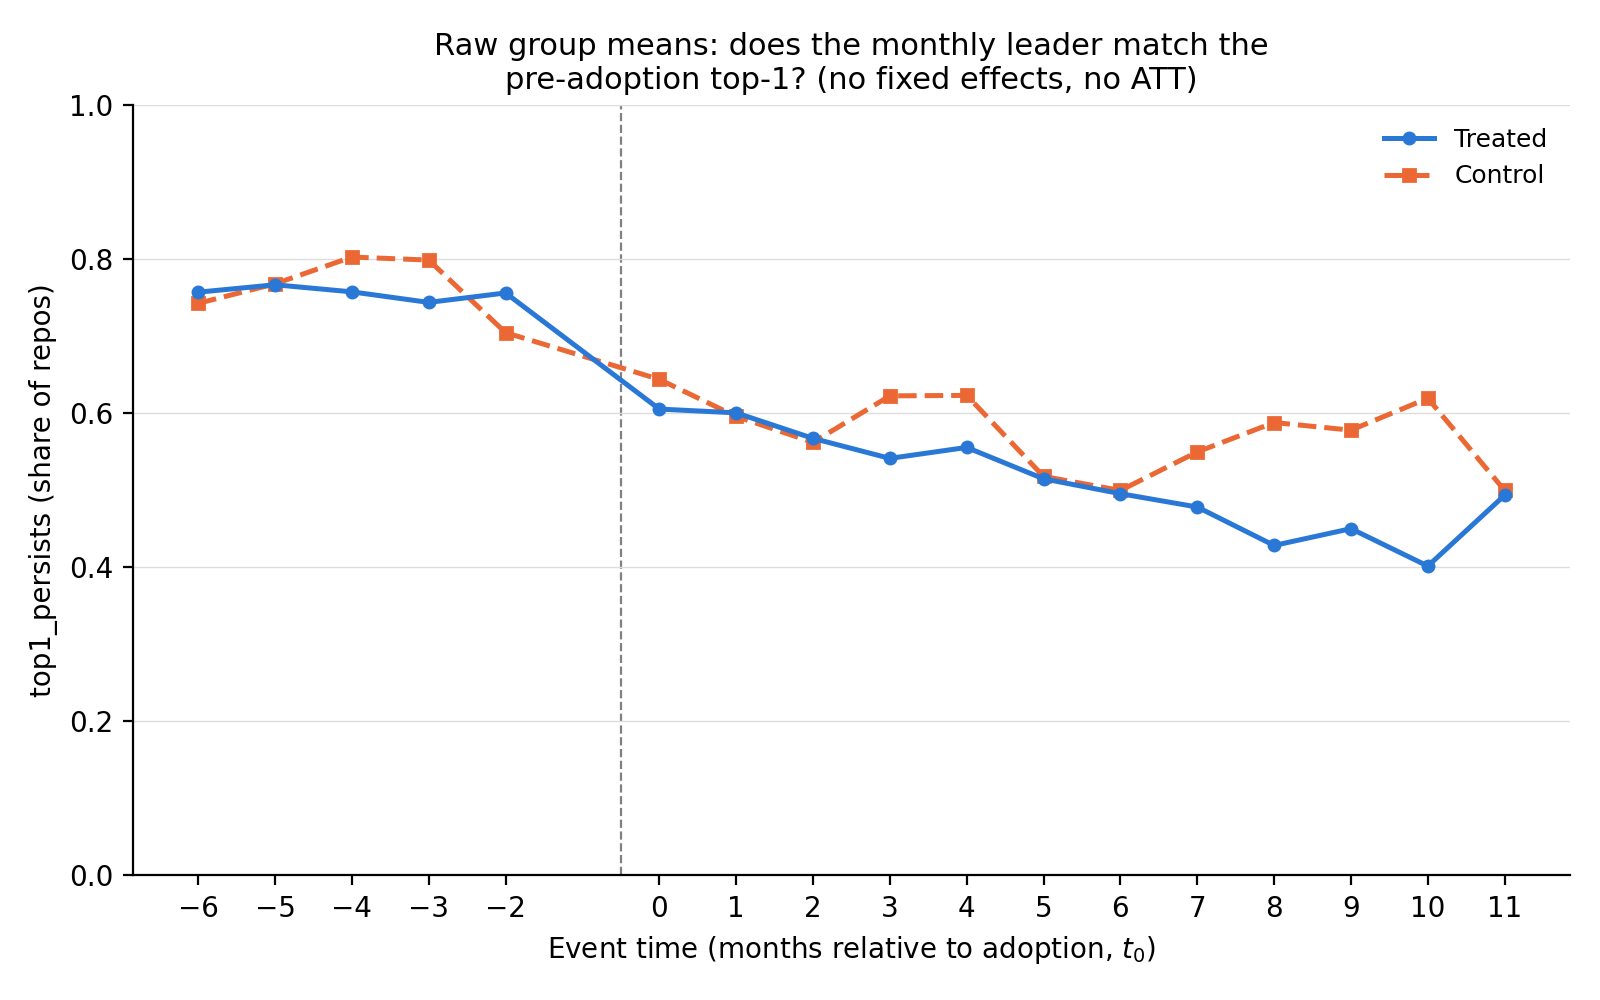
\includegraphics[width=0.62\textwidth]{top1_persists_raw_event_time.png}
\end{center}
\vspace{-0.3em}
\footnotesize Both groups drop from $\sim$0.75 to $\sim$0.60 at
$h\!=\!0$. Because the drop is common to treated and control, the
difference-in-differences nets it out; the series separate only later.
\end{frame}

\begin{frame}{RQ3 --- Process Outcomes}
\begin{table}
\centering
\small
\begin{tabular}{lrr}
\toprule
Outcome & ATT & $p$ \\
\midrule
Time to first review (h) & $-65.0^{*}$ \ (28.91) & 0.025 \\
Time to merge (h)        & $-62.8^{*}$ \ (27.10) & 0.021 \\
Review rounds/PR         & $+0.180^{*}$ \ (0.082) & 0.027 \\
\addlinespace
Repo FE & Yes & \\
Time FE & Yes & \\
\bottomrule
\end{tabular}
\end{table}
\begin{itemize}
  \item PRs reach a first recorded review and merge sooner, while review
        submissions per PR increase.
\end{itemize}
\end{frame}

\begin{frame}{H3 --- Do Pull Requests Just Get Smaller?}
\begin{table}
\centering
\small
\begin{tabular}{lrr}
\toprule
Spec & ATT (hours) & $t$ \\
\midrule
Unrestricted (uncapped PR-level data) & $-34.2$ & $-1.74$ \\
Residualized on PR size & $-35.8$ & $-1.82$ \\
Restricted to similarly-sized PRs (25th--75th pct.) & $-61.8$ & $-2.62$ \\
\bottomrule
\end{tabular}
\end{table}
\begin{itemize}
  \item With PR size held fixed, latency still falls --- merges get
        faster, not merely smaller.
\end{itemize}
\end{frame}

\begin{frame}{H3 --- Reverses in Busy Repos}
On the busier-than-average subsample ($\sim$2$\times$ pre-period PR
volume, $n{=}296$):
\begin{table}
\centering
\small
\begin{tabular}{lrr}
\toprule
Outcome & Full sample & Busy subsample \\
\midrule
Time to merge (h) & $-62.8$ (2.60) & $+40.7$ (2.83) \\
Review rounds/PR & $+0.180$ (4.04) & $-0.146$ (2.04) \\
\bottomrule
\end{tabular}
\end{table}
\begin{itemize}
  \item Both directions pass pre-trends in both samples; the full
        sample's own $\text{ATT}_h$ never flips sign across horizons.
  \item In high-volume repos, merging gets \textbf{slower} and needs
        \textbf{fewer} rounds after adoption, the opposite pattern from
        the general sample.
\end{itemize}
\end{frame}

\section{Discussion}
\begin{frame}{Discussion}
Our results suggest a reallocation of review authority, with important
limits on what the data can identify.
\begin{itemize}
  \item The pre-adoption leader is less likely to remain first after
        adoption, while monthly concentration can rise.
  \item Reassignment is stronger where leadership was not already
        settled, but that pattern is confounded with baseline activity.
  \item The data do not show whether successors have less context or
        whether incumbents face more absolute work.
\end{itemize}
\vspace{0.3em}
The supported claim is a change in observed allocation and continuity,
not a proven loss of expertise or durable authority.
\end{frame}

\begin{frame}{Reconstructing the Process}
The standard pipeline (earlier slide) treats code review as a
discrete gate at the end: write, then check. That shape assumes
writing is the slow, scarce step.
\begin{itemize}
  \item AI-assisted production changes the volume and composition of work
        reaching review, while the organizational response remains an
        empirical question.
  \item The observed evidence points to a change in review allocation and
        incumbent continuity, with substantial sample and measurement
        sensitivity.
  \item The data do not identify whether successors have less context,
        whether incumbents face more absolute work, or whether quality
        improves or declines.
\end{itemize}
\vspace{0.3em}
The supported contribution is a measurement framework for studying
allocation, continuity, and process timing together.
\end{frame}

\begin{frame}{Are Our Controls Actually Independent?}
\textbf{Problem:} 37.7\% of repos share a human reviewer with some
treated repo elsewhere in the sample -- that reviewer can carry
AI-adoption habits into a repo we're counting as an untreated
``control,'' violating the no-interference assumption the design needs.
\vspace{0.3em}

\textbf{What we did:} identified 176 pairs without observed reviewer
overlap and examined the headline outcomes in that restricted sample.
\vspace{0.3em}

\textbf{Result if contamination is removed:}
\begin{itemize}
  \item Top-2 share and incumbent persistence retain their direction;
        the persistence estimate is larger in the restricted sample.
  \item Other outcomes weaken or become imprecise, as expected after the
        population is reduced to 176 pairs.
  \item Month-to-month leader-change rate collapses to $t{\approx}0$ and
        is dropped as a robust claim.
\end{itemize}
\end{frame}

\begin{frame}{Is the Reported Inference Trustworthy?}
Analytic cluster-robust SE vs.\ a 300-replicate repo-pair bootstrap:
\begin{table}
\centering
\scriptsize
\begin{tabular}{lrrrr}
\toprule
Outcome & Analytic SE & Bootstrap SE & Ratio & Corrected $p$ \\
\midrule
Top-1 review share     & 0.0064 & 0.0089 & 1.39$\times$ & 0.052 \\
Top-2 review share     & 0.0034 & 0.0050 & 1.45$\times$ & 0.003 \\
Time to first review   & 21.40  & 28.91  & 1.35$\times$ & 0.025 \\
Time to merge          & 24.18  & 27.10  & 1.12$\times$ & 0.021 \\
Review rounds          & 0.045  & 0.082  & 1.83$\times$ & 0.027 \\
\bottomrule
\end{tabular}
\end{table}
The analytic SE understates true uncertainty by 12--83\%. Top-1 share
drops to borderline ($p=0.052$); everything else survives. All tables
in this deck use the corrected $p$.
\end{frame}

\begin{frame}{The Parallel-Trends Assumption for BJS}
\begin{itemize}
  \item BJS builds each treated repo's counterfactual,
        $\hat\alpha_i+\hat\beta_t$, from a model fit only on
        pre-adoption and control data. That counterfactual is valid
        only if, absent treatment, the repo would have kept following
        that same repo-baseline-plus-calendar-trend path.
  \item Primary check (go/no-go): joint Wald test on the five
        pre-period lead coefficients ($h=-6,\dots,-2$), $\chi^2_5$.
  \item Secondary check (margin of safety): how large an undetected
        pre-trend would need to be, extrapolated forward, to explain
        away the post-period effect --- in units of the estimated
        pre-trend's own SE.
\end{itemize}
\begin{table}
\centering
\tiny
\begin{tabular}{lr}
\toprule
Outcome & Breakdown slope, in SE units \\
\midrule
Top-1 review share     & 2.6$\times$ (wrong-signed pre-trend --- helps us) \\
Top-2 review share     & 3.4$\times$ (wrong-signed pre-trend --- helps us) \\
Time to first review   & 3.7$\times$ (same-signed --- erodes $\sim$36\% of ATT) \\
Time to merge          & 3.8$\times$ \\
Review rounds          & 3.0$\times$ (same-signed --- erodes $\sim$55\% of ATT) \\
\bottomrule
\end{tabular}
\end{table}
\end{frame}

\begin{frame}{Does the Effect Differ by Adoption Era?}
Repos adopted 2025-05 to 2025-11 (``Era 2'', $n{=}413$) vs.\
2025-11 to 2026-05 (``Era 3'', $n{=}666$) -- the two best-powered
calendar-time cohorts, roughly bracketing successive generations of
agentic coding tools:
\begin{table}
\centering
\small
\begin{tabular}{lrrl}
\toprule
Outcome & Era 2 ATT & Era 3 ATT & Diff.\ test \\
\midrule
Top-1 review share & $+0.028$ & $+0.020$ & $p=0.60$ \\
Top-2 review share & $+0.021$ & $+0.014$ & $p=0.42$ \\
\bottomrule
\end{tabular}
\end{table}
\begin{itemize}
  \item No test in a full battery -- caliper sensitivity, bootstrap
        SE, clean-sample restriction -- ever produces a significant
        Era-2-vs-Era-3 difference on this comparison.
  \item \textbf{The effect is not detectably different across adoption
        eras.} Not driven by a specific generation of AI coding tools.
\end{itemize}
\end{frame}

\begin{frame}{Does the Effect Differ by Specific Tool?}
Beyond agent-vs-assisted MODE (earlier slide): does it matter whether a
repo adopted Codex, Copilot, Claude, or Cursor specifically? Buckets are
non-exclusive (a repo can carry signals for more than one tool).
\begin{table}
\centering
\small
\begin{tabular}{lrrr}
\toprule
Tool ($n$) & Top-2 share $t$ & Time-to-merge $t$ \\
\midrule
Codex (961)    & $+1.57$ & $-2.97$ \\
Copilot (800)  & $+3.18$ & $-2.60$ \\
Claude (478)   & $+2.55$ & $-1.26$ \\
Cursor (151)   & $+0.66$ & $+1.10$ \\
\bottomrule
\end{tabular}
\end{table}
\vspace{0.2em}
\textbf{Conclusion:} the concentration result is not detectably different
across adoption eras or specific AI tools; Codex's latency estimate is
individually robust but not larger than the alternatives.
\end{frame}

% \begin{frame}{Robustness: Extraction Cap and Common Horizon}
% \begin{table}
% \centering\small
% \begin{tabular}{lrr}
% \toprule
% Top-two share specification & ATT & Notes \\
% \midrule
% Original capped extraction & $+0.0153$ & full eligible sample \\
% Uncapped extraction & $+0.0082$ & same 802-repository subsample \\
% Full event window & $+0.0151$ & pooled sample \\
% Common horizon $h=0,\ldots,5$ & $+0.0081$ & fixed early window \\
% \bottomrule
% \end{tabular}
% \end{table}
% \begin{itemize}
%   \item Direction is stable, but magnitude depends on the extraction cap
%         and the changing cohort composition at longer horizons.
%   \item The cap and common-horizon checks limit a strong claim about the
%         size of the concentration effect.
% \end{itemize}
% \end{frame}

\begin{frame}{Robustness: No Observed Reviewer Overlap}
\begin{table}
\centering\scriptsize
\begin{tabular}{lrr}
\toprule
Outcome, 176 pairs & ATT & Analytic $t$ \\
\midrule
Top-one share & $+0.0118$ & 0.86 \\
Top-two share & $+0.0208$ & 2.79 \\
Incumbent persistence & $-0.1106$ & $-3.70$ \\
Pre-adoption top-two overlap & $+0.0095$ & 0.45 \\
Monthly leader changes & $-0.0006$ & $-0.02$ \\
First recorded review (h) & $-89.77$ & $-2.92$ \\
Merge time (h) & $-56.15$ & $-1.88$ \\
Review submissions/PR & $+0.1756$ & 1.82 \\
\bottomrule
\end{tabular}
\end{table}
\footnotesize This restriction changes the population and uses analytic
inference, not the pooled table's bootstrap. It removes observed overlap,
not every possible spillover.
\end{frame}


\begin{frame}[plain]
\begin{center}
\Large Thank you
\vspace{1em}

\normalsize Questions?
\end{center}
\end{frame}
.
%
% Active deck contains no bibliography or citation commands.
%
% New figure required:
%   figures/top1_persists_raw_event_time.png
%   (raw group means of top1_persists by event time, treated vs control)
%
% Claims deliberately removed because the data does not support them:
%   "fewer hands" / "review lands on fewer people"  -> n_reviewers is null
%   "single point of failure"                       -> top1_persists falls
% =========================================================================

\section{Motivation}

\begin{frame}{AI Changes Software Production}
\begin{itemize}
  \item RCT evidence: developers using GitHub Copilot completed a
        standardized coding task 55.8\% faster than a control group
        .
  \item Enterprise RCT: 96 Google engineers on a complex,
        enterprise-grade C++ task were about 21\% faster with AI
        assistance .
  \item Field and multi-firm evidence points the same way
        .
  \item These results motivate a production question rather than a
        universal productivity premise: what happens to code review work?
\end{itemize}
\end{frame}

\begin{frame}{The Code Review Problem}
\begin{itemize}
  \item Faster authoring means more code arriving at the review gate,
        while review itself stays human work.
  \item That code is not trustworthy by default. Across 54
        security-relevant scenarios, 44\% of the 1,084 valid programs
        Copilot produced contained a MITRE CWE
        .
  \item In a controlled user study, participants with an AI assistant
        wrote significantly less secure code than those without --- and
        were likelier to believe their code was secure
        .
  \item Bird et al.\ (GitHub / Microsoft Research) describe the same
        shift from the inside: effort moves from writing code toward
        reviewing it .
\end{itemize}
\end{frame}

\begin{frame}{Standard Pipeline}
\begin{center}
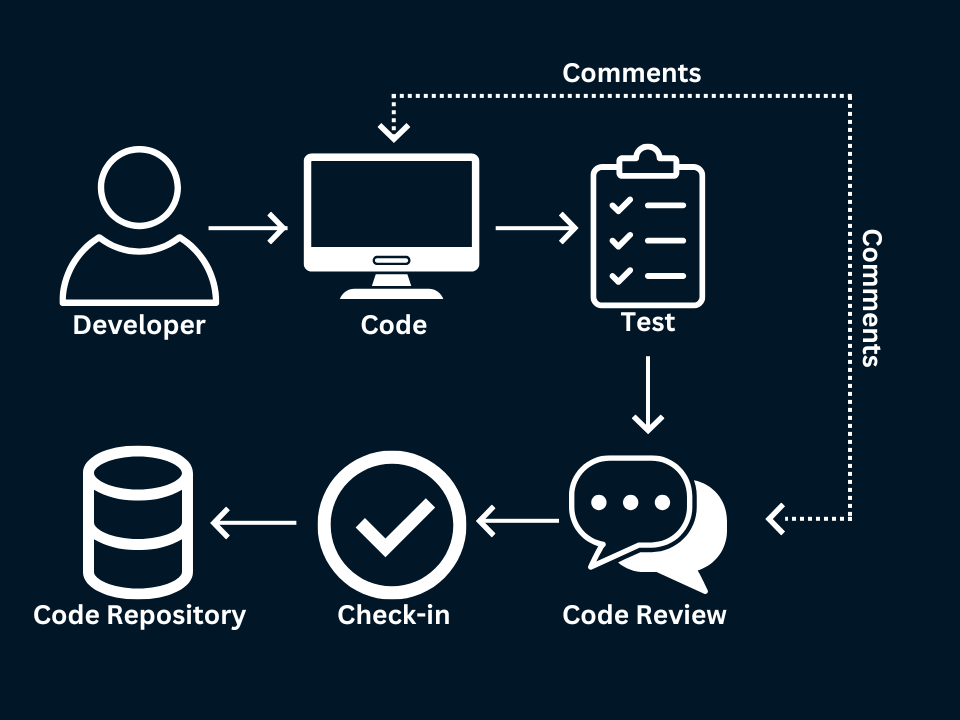
\includegraphics[width=0.6\textwidth]{code_process.png}
\end{center}
\footnotesize\centering 
Code review is where generated changes meet project knowledge,
governance, and coordination. The question is how review activity is
allocated after adoption.
\end{frame}

\section{Literature Review}

\begin{frame}{Related Work: Team-Level Effects Already Documented}
\begin{itemize}
  \item Review depth rises 5.3\% in a matched staggered-DiD study of
        11,097 repositories .
  \item Human reviewers exchange 11.8\% more rounds reviewing
        AI-generated code .
  \item An enterprise throughput mandate roughly doubles per-reviewer
        load .
\end{itemize}
\end{frame}

\begin{frame}{Related Work: Team Coordination Specifically}
\begin{itemize}
  \item AI access shifts developer time away from collaborative and
        management tasks toward solo coding, strongest for lower-skill
        developers .
  \item At Meta, lines of code per human-landed diff rose 105.9\%
        year-over-year, driven substantially by agentic AI --- review
        demand is outpacing reviewer bandwidth .
  \item Governance of AI-assisted contributions varies sharply: many
        AI-co-authored PRs merge with minimal or no human review
        .
  \item Across 1.02M pull requests, agent-involved review is faster but
        not higher-quality .
\end{itemize}
\end{frame}

\begin{frame}{Related Work: The Narrow Gap}
Closest comparator: Copilot adoption raises project-level contributions
5.9\% and coordination time 8\%; core-developer reviews, reviews per
core developer, and distinct core reviewers all rise
.
\vspace{0.3em}
\textbf{The remaining question here:}
\begin{itemize}
  \item Project-level averages and counts do not reveal the distribution
        of review activity across people.
  \item Monthly concentration and fixed reviewer identity are distinct:
        the busiest people can change while concentration stays constant.
  \item We study review-share concentration jointly with continuity of
        the people occupying leading review positions.
\end{itemize}
\end{frame}

\section{Theory}

% \begin{frame}{Review as a Transactive Memory System}
% A transactive memory system (TMS) is a group's shared directory of
% \emph{who knows what} -- members specialize, and the group knows whom
% to route a problem to .
% \begin{itemize}
%   \item In software, that directory is built from accumulated codebase
%         memory: why a decision was made, what broke before.
%   \item Review is where it's exercised -- who reviews what determines
%         what gets caught.
%   \item Open-source review makes it \textbf{observable}: assignment is
%         recorded behaviour, not survey data.
% \end{itemize}
% \vspace{0.3em}
% TMS separates two things the throughput literature conflates: how
% \emph{specialized} code review is, and \emph{whom} it's specialized
% onto.
% \end{frame}



% \begin{frame}{The Review Process, Before AI}
% \begin{center}
% 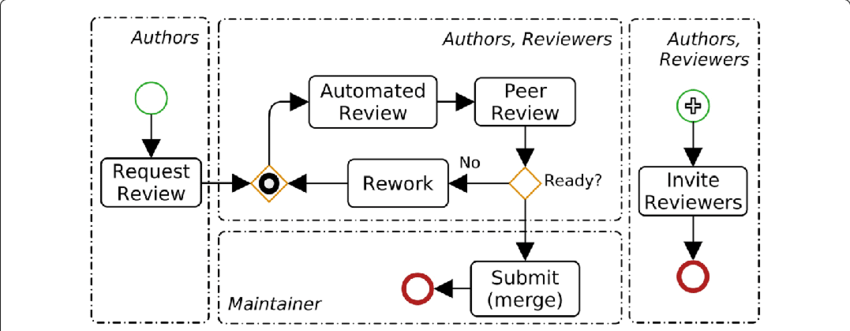
\includegraphics[width=0.78\textwidth]{review_process.png}
% \end{center}
% \footnotesize\centering Inside ``Code Review''
% \\
% \vspace{0.5em}
% \end{frame}

\begin{frame}{Research Questions}
\textbf{Question:} when a repository first exhibits an AI-adoption
signal, how does its review work reorganize?
\begin{enumerate}
  \item[RQ1] Does the distribution of monthly review activity change?
  \item[RQ2] Does the pre-adoption leading reviewer remain in the leading
        position, and what happens to successor stability?
  \item[RQ3] What process outcomes accompany these allocation patterns?
\end{enumerate}
\end{frame}

\section{Research Design and Data}

\begin{frame}{Research Design}
\begin{itemize}
  \item Treatment: a repository's own AI-tool adoption, $t_0$ =
        earliest detected signal.
  \item Staggered-adoption DiD on covariate-matched treated/control
        repositories.
  \item Imputation estimator of  ---
        avoids the ``forbidden comparisons'' bias of naive two-way
        fixed effects under staggered timing
        .
  \item 1,771 matched pairs, 20,188 repository-month observations.
\end{itemize}
\end{frame}

\begin{frame}{Data Construction}
\begin{itemize}
  \item 8,972 candidate repositories, stratified across 6 languages
        $\times$ 4 creation-year cohorts, quality-filtered ($\geq$10
        stars, not a fork, minimum contributor count, recent activity
        ).
  \item AI-adoption signal (OR-combined): autonomous agent PR
        authorship, commit co-authorship trailers, configuration-file
        presence. $t_0$ = first detected signal of any kind.
  \item[] 8,972 candidates $\rightarrow$ 2,320 matched pairs (caliper
        0.25 SD) $\rightarrow$ 1,771 pairs with complete panel data.
\end{itemize}
\end{frame}

\begin{frame}{Outcome Variables}
Each measured per repository-month; construction detail in backup.
\begin{itemize}
  \item \textbf{Specialization:} top1\_share/top2\_share -- the busiest
        one/two reviewers' share of a repo-month's total human review
        activity; tail\_share is the complement held by everyone else.
  \item \textbf{Directory assignment:} top1\_persists: is this month's
        busiest reviewer the same person as the repository's fixed
        pre-period top-1? Same for the top-2 pair.
\end{itemize}
\end{frame}

\begin{frame}{Outcome Variables}
Gini coefficient over a repo-month's full reviews-per-reviewer
distribution: 
\[
G_{it}=\frac{\displaystyle\sum_{r=1}^{n}\sum_{q=1}^{n}
\left|x_{rit}-x_{qit}\right|}
{\displaystyle 2n\sum_{r=1}^{n}x_{rit}}
\]
\begin{itemize}
  \item $x_i$ = number of reviews reviewer $i$ submitted that
        repo-month; $n$ = number of distinct human reviewers that
        repo-month.
  \item G = 0 mean every reviewer handled an equal share.
  \item G = 1 mean one reviewer handled all of it.
\end{itemize}
\end{frame}

\section{Empirical Strategy}

\begin{frame}{Introducing BJS: Why We Need It}
\begin{itemize}
  \item Repos adopt AI at different times --- naive two-way fixed
        effects implicitly compares late adopters against
        already-treated early adopters, not just never-treated
        controls.
  \item These ``forbidden comparisons'' bias the estimate whenever the
        treatment effect changes over time
         --- exactly our case, since our
        effects grow across the post-period.
  \item We use the imputation estimator of
         (``BJS''): it builds each treated
        repo's counterfactual only from never-yet-treated data, so an
        already-treated repo can never contaminate another's
        comparison.
\end{itemize}
\end{frame}

\begin{frame}{Estimator}
Two-step imputation :
\begin{enumerate}
  \item Fit $y_{it}=\alpha_i+\beta_t+\varepsilon_{it}$ on $\Omega_0$
        (controls' full history + treated repos' pre-$t_0$
        observations only).
  \item Predict $\hat y_{it}(0)=\hat\alpha_i+\hat\beta_t$ for treated
        post-$t_0$ observations; $\text{ATT}_h$ = mean residual at
        event-time horizon $h$.
\end{enumerate}
\vspace{0.5em}
Event time: pre-leads $h=-6,\dots,-2$ (no-anticipation: $h=-1$
excluded), post-period $h=0,\dots,11$.
\vspace{0.5em}
Post-adoption data = a treated repo's own observations after its $t_0$.
Step 1 never uses it.
\end{frame}

\begin{frame}{BJS in Practice: Observed vs.\ Counterfactual}
\begin{center}
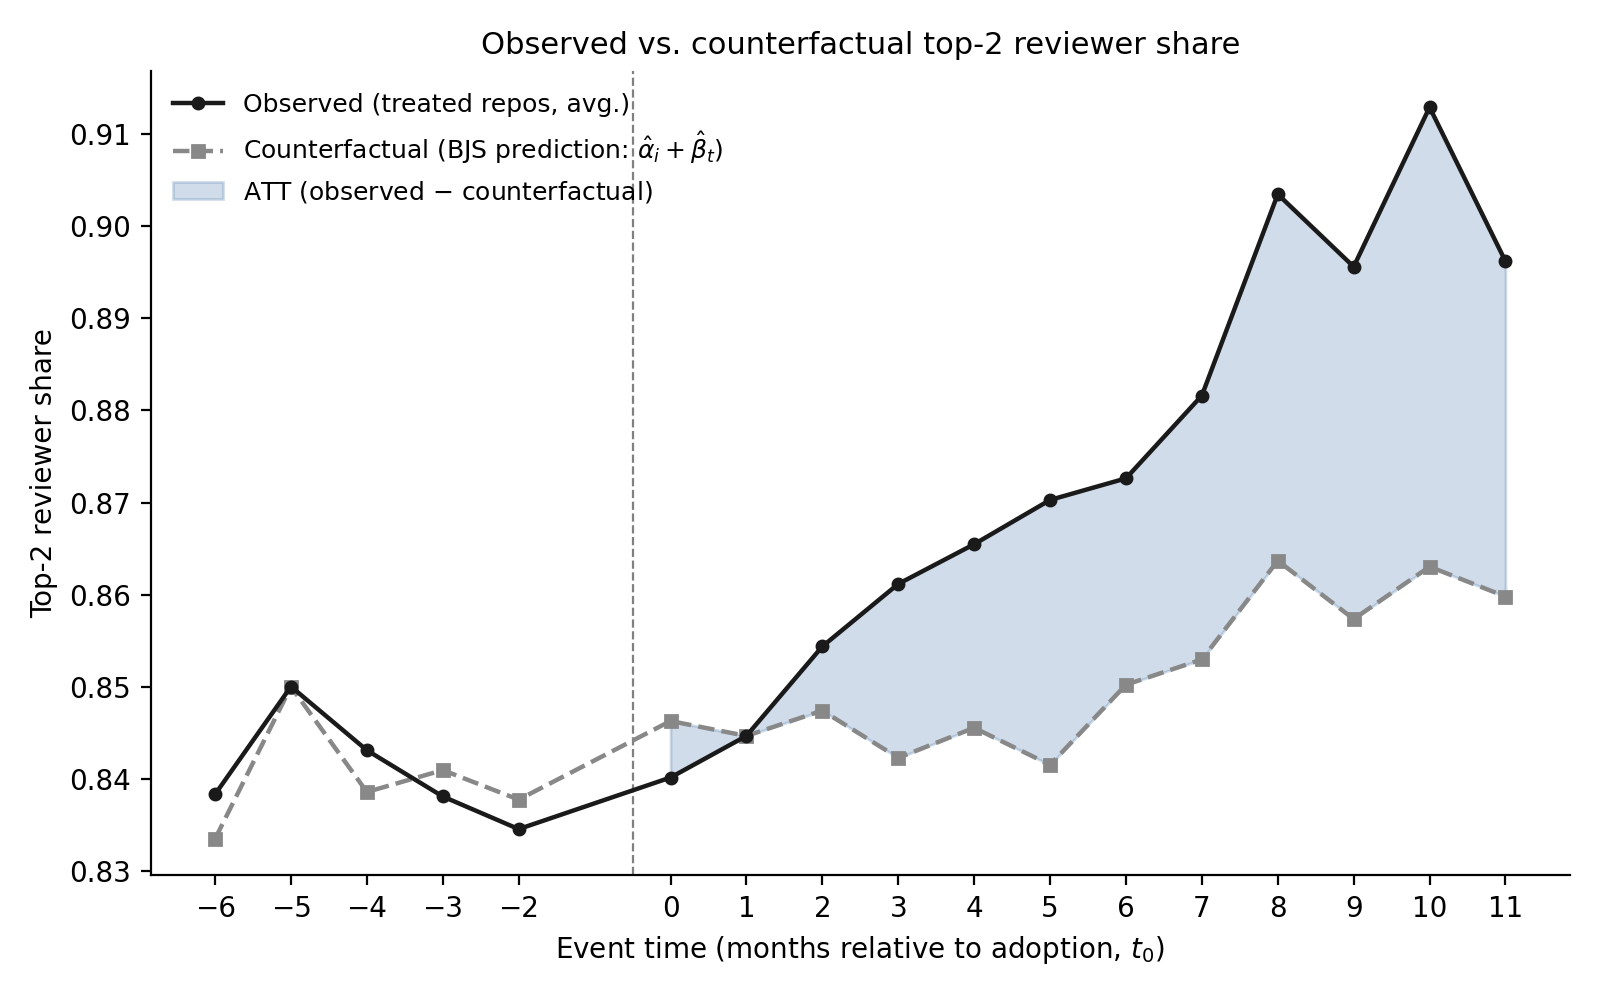
\includegraphics[width=0.85\textwidth]{bjs_illustration_top2_share.png}
\end{center}
\end{frame}

\section{Results}

\begin{frame}{RQ1 --- Monthly Review Activity Becomes More Concentrated}
\begin{table}
\centering
\small
\begin{tabular}{lrr}
\toprule
Outcome & ATT & $p$ \\
\midrule
Top-1 review share & $+0.017$ \ (0.0089) & 0.052 \\
Top-2 review share & $+0.015^{**}$ \ (0.0050) & 0.003 \\
Tail share (outside the top two) & $-0.015^{***}$ & $<0.001$ \\
Reviewer Gini coefficient & $+0.030^{***}$ & $<0.001$ \\
\addlinespace
\multicolumn{3}{l}{\textit{Repos with 3+ reviewers monthly}} \\
Top-1 review share & $+0.041^{***}$ \ (0.0072) & $<0.001$ \\
Top-2 review share & $+0.036^{***}$ \ (0.0052) & $<0.001$ \\
\addlinespace
Repo FE & Yes & \\
Time FE & Yes & \\
\bottomrule
\end{tabular}
\end{table}
\end{frame}

\begin{frame}{RQ1 --- What the Numbers Show}
\begin{itemize}
  \item \textbf{Headcount:} team size is unchanged in this outcome -- the
        observed distribution changes within the measured reviewer set.
  \item \textbf{Concentration:} top-2 share rises while tail share falls
        by almost the same amount, and the Gini rises across the whole
        distribution.
  \item Many repo-months start pinned near 100\% (only 1--2 reviewers),
        diluting the pooled estimate; restricting to 3+ reviewers
        roughly doubles it.
\end{itemize}
\vspace{0.3em}
\end{frame}

\begin{frame}{RQ1 --- Concentration Depends on Whether Leadership Was Already Settled}
Split treated repos by whether one person already held the top spot for
the entire 5-month pre-period (``settled'') or not (``unsettled''):
\begin{table}
\centering
\small
\begin{tabular}{lrr}
\toprule
Outcome & Unsettled leader ($n{=}191$) & Settled leader ($n{=}105$) \\
\midrule
Top-1 review share & $+0.047$ (4.62) & $-0.022$ ($-1.84$) \\
Top-2 review share & $+0.036$ (4.40) & $+0.001$ (0.14) \\
\bottomrule
\end{tabular}
\end{table}
\begin{itemize}
  \item Both strata pass pre-trend cleanly; the difference between them
        is strongly significant (top-1: $p<0.0001$, top-2: $p=0.003$).
  \item \textbf{Scope:} this subsample (complete 5-month pre-period
        coverage) also skews busier than average ($\sim$2$\times$ the
        pre-period PR volume)
\end{itemize}
\end{frame}

\begin{frame}{RQ2 --- Incumbent Persistence Falls}
\begin{table}
\centering
\small
\begin{tabular}{lrr}
\toprule
Outcome & ATT & $p$ \\
\midrule
Monthly leader is the pre-adoption top-1 & $-0.077^{***}$ \ (0.0151) & $<0.001$ \\
Monthly top-2 overlaps the pre-adoption top-2 & $-0.045^{***}$ \ (0.0101) & $<0.001$ \\
Month-to-month leader change & $-0.058^{**}$ \ (0.0197) & 0.004 \\
\addlinespace
Repo FE & Yes & \\
Time FE & Yes & \\
\bottomrule
\end{tabular}
\end{table}
\begin{itemize}
  \item The pre-adoption lead is less likely to remain the monthly leader
        after adoption.
\end{itemize}
\end{frame}

\begin{frame}{RQ2 --- Is the Persistence Result a Construction Artifact?}
The fixed identity is chosen by taking the maximum over
$h=-6,\dots,-2$, and those same months form the estimation baseline ---
which inflates pre-period persistence by construction.
\begin{center}
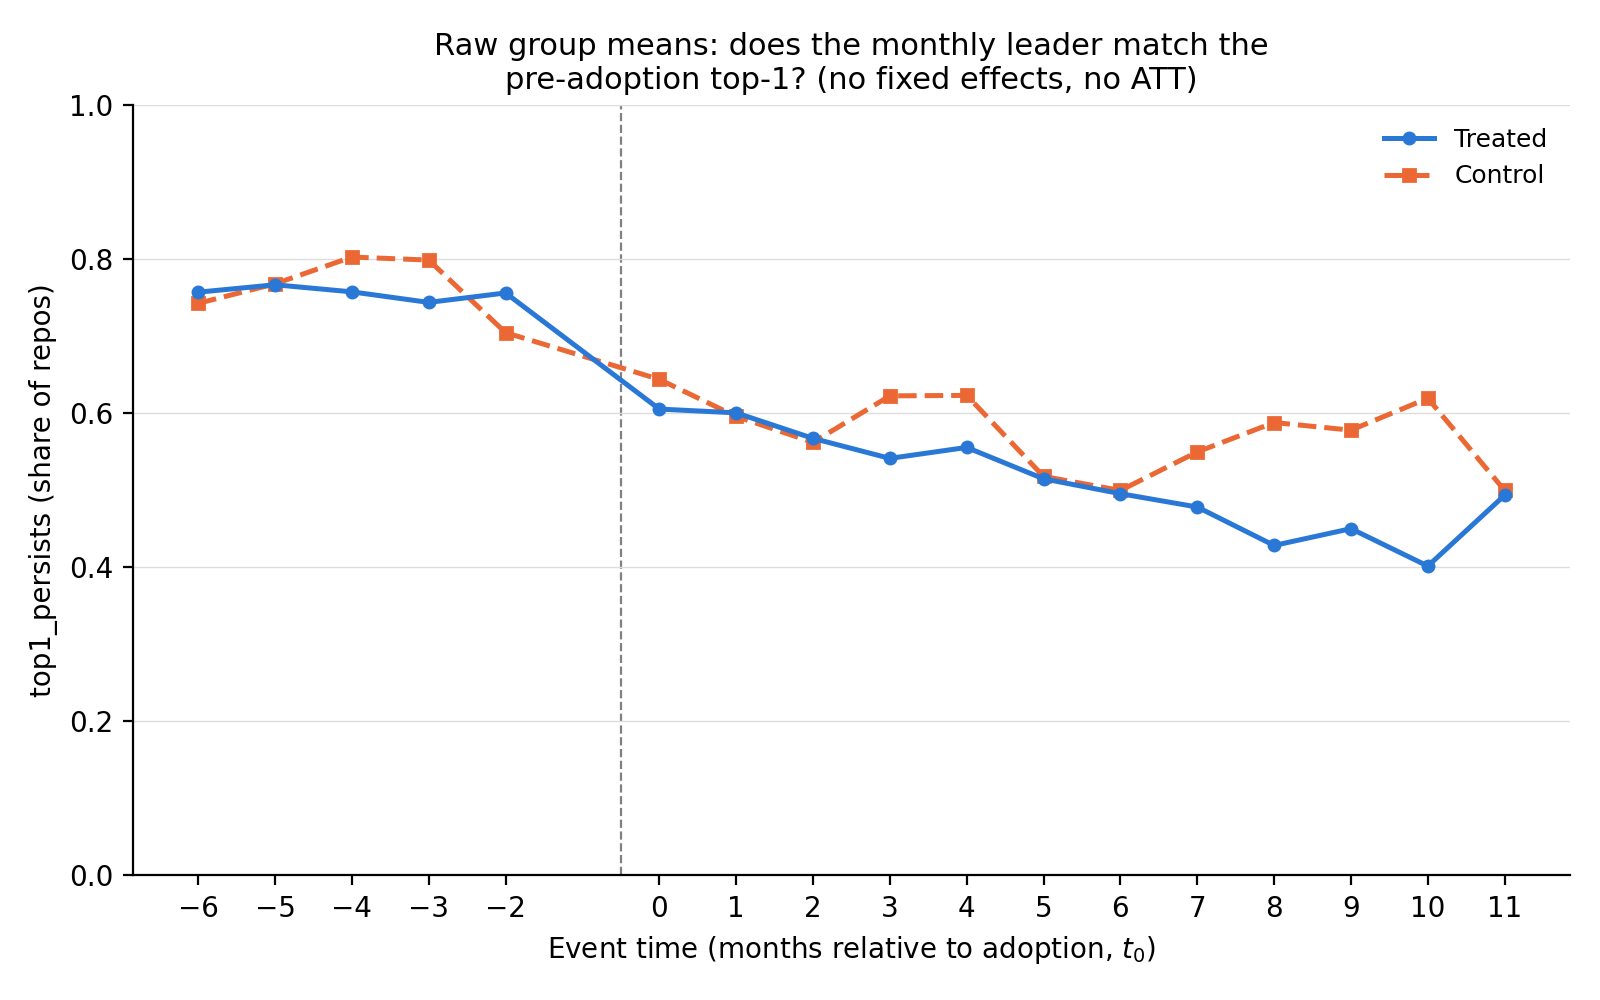
\includegraphics[width=0.62\textwidth]{top1_persists_raw_event_time.png}
\end{center}
\vspace{-0.3em}
\footnotesize Both groups drop from $\sim$0.75 to $\sim$0.60 at
$h\!=\!0$. Because the drop is common to treated and control, the
difference-in-differences nets it out; the series separate only later.
\end{frame}

\begin{frame}{RQ3 --- Process Outcomes}
\begin{table}
\centering
\small
\begin{tabular}{lrr}
\toprule
Outcome & ATT & $p$ \\
\midrule
Time to first review (h) & $-65.0^{*}$ \ (28.91) & 0.025 \\
Time to merge (h)        & $-62.8^{*}$ \ (27.10) & 0.021 \\
Review rounds/PR         & $+0.180^{*}$ \ (0.082) & 0.027 \\
\addlinespace
Repo FE & Yes & \\
Time FE & Yes & \\
\bottomrule
\end{tabular}
\end{table}
\begin{itemize}
  \item PRs reach a first recorded review and merge sooner, while review
        submissions per PR increase.
\end{itemize}
\end{frame}

\begin{frame}{H3 --- Do Pull Requests Just Get Smaller?}
\begin{table}
\centering
\small
\begin{tabular}{lrr}
\toprule
Spec & ATT (hours) & $t$ \\
\midrule
Unrestricted (uncapped PR-level data) & $-34.2$ & $-1.74$ \\
Residualized on PR size & $-35.8$ & $-1.82$ \\
Restricted to similarly-sized PRs (25th--75th pct.) & $-61.8$ & $-2.62$ \\
\bottomrule
\end{tabular}
\end{table}
\begin{itemize}
  \item With PR size held fixed, latency still falls --- merges get
        faster, not merely smaller.
\end{itemize}
\end{frame}

\begin{frame}{H3 --- Reverses in Busy Repos}
On the busier-than-average subsample ($\sim$2$\times$ pre-period PR
volume, $n{=}296$):
\begin{table}
\centering
\small
\begin{tabular}{lrr}
\toprule
Outcome & Full sample & Busy subsample \\
\midrule
Time to merge (h) & $-62.8$ (2.60) & $+40.7$ (2.83) \\
Review rounds/PR & $+0.180$ (4.04) & $-0.146$ (2.04) \\
\bottomrule
\end{tabular}
\end{table}
\begin{itemize}
  \item Both directions pass pre-trends in both samples; the full
        sample's own $\text{ATT}_h$ never flips sign across horizons.
  \item In high-volume repos, merging gets \textbf{slower} and needs
        \textbf{fewer} rounds after adoption, the opposite pattern from
        the general sample.
\end{itemize}
\end{frame}

\section{Discussion}
\begin{frame}{Discussion}
Our results suggest a reallocation of review authority, with important
limits on what the data can identify.
\begin{itemize}
  \item The pre-adoption leader is less likely to remain first after
        adoption, while monthly concentration can rise.
  \item Reassignment is stronger where leadership was not already
        settled, but that pattern is confounded with baseline activity.
  \item The data do not show whether successors have less context or
        whether incumbents face more absolute work.
\end{itemize}
\vspace{0.3em}
The supported claim is a change in observed allocation and continuity,
not a proven loss of expertise or durable authority.
\end{frame}

\begin{frame}{Reconstructing the Process}
The standard pipeline (earlier slide) treats code review as a
discrete gate at the end: write, then check. That shape assumes
writing is the slow, scarce step.
\begin{itemize}
  \item AI-assisted production changes the volume and composition of work
        reaching review, while the organizational response remains an
        empirical question.
  \item The observed evidence points to a change in review allocation and
        incumbent continuity, with substantial sample and measurement
        sensitivity.
  \item The data do not identify whether successors have less context,
        whether incumbents face more absolute work, or whether quality
        improves or declines.
\end{itemize}
\vspace{0.3em}
The supported contribution is a measurement framework for studying
allocation, continuity, and process timing together.
\end{frame}

\begin{frame}{Are Our Controls Actually Independent?}
\textbf{Problem:} 37.7\% of repos share a human reviewer with some
treated repo elsewhere in the sample -- that reviewer can carry
AI-adoption habits into a repo we're counting as an untreated
``control,'' violating the no-interference assumption the design needs.
\vspace{0.3em}

\textbf{What we did:} identified 176 pairs without observed reviewer
overlap and examined the headline outcomes in that restricted sample.
\vspace{0.3em}

\textbf{Result if contamination is removed:}
\begin{itemize}
  \item Top-2 share and incumbent persistence retain their direction;
        the persistence estimate is larger in the restricted sample.
  \item Other outcomes weaken or become imprecise, as expected after the
        population is reduced to 176 pairs.
  \item Month-to-month leader-change rate collapses to $t{\approx}0$ and
        is dropped as a robust claim.
\end{itemize}
\end{frame}

\begin{frame}{Is the Reported Inference Trustworthy?}
Analytic cluster-robust SE vs.\ a 300-replicate repo-pair bootstrap:
\begin{table}
\centering
\scriptsize
\begin{tabular}{lrrrr}
\toprule
Outcome & Analytic SE & Bootstrap SE & Ratio & Corrected $p$ \\
\midrule
Top-1 review share     & 0.0064 & 0.0089 & 1.39$\times$ & 0.052 \\
Top-2 review share     & 0.0034 & 0.0050 & 1.45$\times$ & 0.003 \\
Time to first review   & 21.40  & 28.91  & 1.35$\times$ & 0.025 \\
Time to merge          & 24.18  & 27.10  & 1.12$\times$ & 0.021 \\
Review rounds          & 0.045  & 0.082  & 1.83$\times$ & 0.027 \\
\bottomrule
\end{tabular}
\end{table}
The analytic SE understates true uncertainty by 12--83\%. Top-1 share
drops to borderline ($p=0.052$); everything else survives. All tables
in this deck use the corrected $p$.
\end{frame}

\begin{frame}{The Parallel-Trends Assumption for BJS}
\begin{itemize}
  \item BJS builds each treated repo's counterfactual,
        $\hat\alpha_i+\hat\beta_t$, from a model fit only on
        pre-adoption and control data. That counterfactual is valid
        only if, absent treatment, the repo would have kept following
        that same repo-baseline-plus-calendar-trend path.
  \item Primary check (go/no-go): joint Wald test on the five
        pre-period lead coefficients ($h=-6,\dots,-2$), $\chi^2_5$.
  \item Secondary check (margin of safety): how large an undetected
        pre-trend would need to be, extrapolated forward, to explain
        away the post-period effect --- in units of the estimated
        pre-trend's own SE.
\end{itemize}
\begin{table}
\centering
\tiny
\begin{tabular}{lr}
\toprule
Outcome & Breakdown slope, in SE units \\
\midrule
Top-1 review share     & 2.6$\times$ (wrong-signed pre-trend --- helps us) \\
Top-2 review share     & 3.4$\times$ (wrong-signed pre-trend --- helps us) \\
Time to first review   & 3.7$\times$ (same-signed --- erodes $\sim$36\% of ATT) \\
Time to merge          & 3.8$\times$ \\
Review rounds          & 3.0$\times$ (same-signed --- erodes $\sim$55\% of ATT) \\
\bottomrule
\end{tabular}
\end{table}
\end{frame}

\begin{frame}{Does the Effect Differ by Adoption Era?}
Repos adopted 2025-05 to 2025-11 (``Era 2'', $n{=}413$) vs.\
2025-11 to 2026-05 (``Era 3'', $n{=}666$) -- the two best-powered
calendar-time cohorts, roughly bracketing successive generations of
agentic coding tools:
\begin{table}
\centering
\small
\begin{tabular}{lrrl}
\toprule
Outcome & Era 2 ATT & Era 3 ATT & Diff.\ test \\
\midrule
Top-1 review share & $+0.028$ & $+0.020$ & $p=0.60$ \\
Top-2 review share & $+0.021$ & $+0.014$ & $p=0.42$ \\
\bottomrule
\end{tabular}
\end{table}
\begin{itemize}
  \item No test in a full battery -- caliper sensitivity, bootstrap
        SE, clean-sample restriction -- ever produces a significant
        Era-2-vs-Era-3 difference on this comparison.
  \item \textbf{The effect is not detectably different across adoption
        eras.} Not driven by a specific generation of AI coding tools.
\end{itemize}
\end{frame}

\begin{frame}{Does the Effect Differ by Specific Tool?}
Beyond agent-vs-assisted MODE (earlier slide): does it matter whether a
repo adopted Codex, Copilot, Claude, or Cursor specifically? Buckets are
non-exclusive (a repo can carry signals for more than one tool).
\begin{table}
\centering
\small
\begin{tabular}{lrrr}
\toprule
Tool ($n$) & Top-2 share $t$ & Time-to-merge $t$ \\
\midrule
Codex (961)    & $+1.57$ & $-2.97$ \\
Copilot (800)  & $+3.18$ & $-2.60$ \\
Claude (478)   & $+2.55$ & $-1.26$ \\
Cursor (151)   & $+0.66$ & $+1.10$ \\
\bottomrule
\end{tabular}
\end{table}
\vspace{0.2em}
\textbf{Conclusion:} the concentration result is not detectably different
across adoption eras or specific AI tools; Codex's latency estimate is
individually robust but not larger than the alternatives.
\end{frame}

% \begin{frame}{Robustness: Extraction Cap and Common Horizon}
% \begin{table}
% \centering\small
% \begin{tabular}{lrr}
% \toprule
% Top-two share specification & ATT & Notes \\
% \midrule
% Original capped extraction & $+0.0153$ & full eligible sample \\
% Uncapped extraction & $+0.0082$ & same 802-repository subsample \\
% Full event window & $+0.0151$ & pooled sample \\
% Common horizon $h=0,\ldots,5$ & $+0.0081$ & fixed early window \\
% \bottomrule
% \end{tabular}
% \end{table}
% \begin{itemize}
%   \item Direction is stable, but magnitude depends on the extraction cap
%         and the changing cohort composition at longer horizons.
%   \item The cap and common-horizon checks limit a strong claim about the
%         size of the concentration effect.
% \end{itemize}
% \end{frame}

\begin{frame}{Robustness: No Observed Reviewer Overlap}
\begin{table}
\centering\scriptsize
\begin{tabular}{lrr}
\toprule
Outcome, 176 pairs & ATT & Analytic $t$ \\
\midrule
Top-one share & $+0.0118$ & 0.86 \\
Top-two share & $+0.0208$ & 2.79 \\
Incumbent persistence & $-0.1106$ & $-3.70$ \\
Pre-adoption top-two overlap & $+0.0095$ & 0.45 \\
Monthly leader changes & $-0.0006$ & $-0.02$ \\
First recorded review (h) & $-89.77$ & $-2.92$ \\
Merge time (h) & $-56.15$ & $-1.88$ \\
Review submissions/PR & $+0.1756$ & 1.82 \\
\bottomrule
\end{tabular}
\end{table}
\footnotesize This restriction changes the population and uses analytic
inference, not the pooled table's bootstrap. It removes observed overlap,
not every possible spillover.
\end{frame}


\begin{frame}[plain]
\begin{center}
\Large Thank you
\vspace{1em}

\normalsize Questions?
\end{center}
\end{frame}

\end{document}
